\documentclass[a4paper]{report}

%----------------------------------------------------------------------------------------
%	PRE-DOCUMENT PAGES
%----------------------------------------------------------------------------------------
%
%\makeglossaries
%
%\graphicspath{{img/}}
%\setmarginsrb{3 cm}{2.5 cm}{3 cm}{2.5 cm}{1 cm}{1.5 cm}{1 cm}{1.5 cm}

%----------------------------------------------------------------------------------------
%	LATEX BUILD INFO
%----------------------------------------------------------------------------------------

%!TEX root = report.tex
\usepackage{color}
%\usepackage{enumitem}
\usepackage{datetime}
\usepackage{courier}
\usepackage{titlesec}
\usepackage{longtable}
% \usepackage{float}
\usepackage[hidelinks]{hyperref}
\usepackage{booktabs}
\usepackage[table,xcdraw,svgnames]{xcolor}
\usepackage{listings}
\usepackage{fancyhdr}

%remove the blank page while using landscape:
\usepackage{afterpage}

\usepackage[]{floatpag}

\usepackage[hypcap]{caption}
%\usepackage{natbib}
%\usepackage{url}
%\usepackage[utf8x]{inputenc}
%\usepackage{amsmath}
%\usepackage{graphicx}
%\usepackage{parskip}
%\usepackage{fancyhdr}
%\usepackage{vmargin}
%\usepackage{xcolor}
%\usepackage{nameref}
%
%\usepackage[hypcap]{caption}

%to reference multiple things at once:
%like \cref{fig:1, fig:2}
%\usepackage{cleveref}

%to frame text with a border
\usepackage{framed}

%to rotate images
\usepackage{rotating}
%usd to cite multiple things at once
% like \cite{citate1, citate2}
%\usepackage{cite}

%used to create lists without any spacing
\usepackage{adjustbox}

%to serperate the table style from the data
\usepackage{pgfplotstable}

%to make a compact itemize list in a table
%\usepackage{paralist}


% To make the table captions on top
\let\newfloat\relax
\usepackage{floatrow}
\floatsetup[table]{capposition=top}

% Accept é ë etc
\usepackage[utf8]{inputenc}
\usepackage[T1]{fontenc}
% Thanks, Laura Baakman

%Show todonotes:
%\usepackage{todonotes}
%Hide todonotes:
\usepackage[disable]{todonotes}

% For shoing euro currency
\usepackage[gen]{eurosym}

%%%%
\usepackage{selinput}
\usepackage[margin=2cm]{geometry}
\usepackage{enumitem,varwidth}
\usepackage{tikz}
\usetikzlibrary{shapes.geometric}
\usepackage{lmodern}
%%%%%%

% parskip puts a lot more white space in to the paper
% I (Guus) prefer it as it allows me te distinguish text
% way faster. However, it's preference, so we could 
% also remove it, if people feel that is needed
\usepackage{parskip}

\usepackage{pbox}
\usepackage[toc]{appendix}

% These packages are used for rotating table header
\usepackage{array}
\usepackage{graphicx}
\usepackage{booktabs}
\usepackage{pifont}

% To determine if a space is needed or not
\usepackage{xspace}
\usepackage{amsmath}

\usepackage[nonumberlist, acronym]{glossaries}


%remove the blank page while using landscape:
\usepackage{afterpage}

% For landscape page
\usepackage{pdflscape}
%!TEX root = report.tex
\newcommand{\todonote}[1]{\textcolor{red}{#1}}
\newcommand{\attention}[1]{\textcolor{green}{#1}}
\newcommand{\HRule}{\rule{\linewidth}{0.5mm}}
\newcommand{\cellBox}[1]{\pbox{0.6\textwidth}{#1}}
\newcommand\myworries[1]{\textcolor{red}{#1}}
\newcommand{\ign}[1]{}

% Commands for rotating table header
\newcommand*\rot{\rotatebox{90}}
\newcommand*\OK{\ding{51}}

\newcommand{\compactCell}[1]{%
    \adjustbox{valign=t}{%
        \begin{minipage}{\linewidth}%
            #1%
        \end{minipage}%
    }%
}

\newcommand{\compactList}[2]{%
    %\begin{minipage}[t][][p]{\linewidth}%
    %\begin{minipage}{\linewidth}%
    \adjustbox{valign=t}{%
        \begin{minipage}{\linewidth}
            \begin{#1}[%
                nosep,
                nolistsep,
                topsep=1pt,
                partopsep=0pt,
                parsep=0pt,
                %itemsep=0pt,
                itemindent=0pt,
                %labelsep=*,
                %align=margin,
                align=left,
                %leftmargin=\linewidth,
                leftmargin=*,
                labelwidth=*,
                after=\strut,
                ]#2\end{#1}%
        \end{minipage}%
    }%\end{adjustbox}
}%

\newcommand{\allotOfText}{%
    LaTeX styled as LATEX, and a shortening of Lamport TeX is a word processor and a document markup language. It is distinguished from typical word processors such as Microsoft Word and Apple Pages in that the writer uses plain text as opposed to formatted text, relying on markup tagging conventions to define the general structure of a document (such as article, book, and letter), to stylise text throughout a document (such as bold and italic), and to add citations and cross-referencing. A TeX distribution such as TeXlive or MikTeX is used to produce an output file (such as PDF or DVI) suitable for printing or digital distribution.
}
%
%\newcolumntype{R}[2]{%
%    >{\adjustbox{angle=#1,lap=\width-(#2)}\bgroup}%
%    l%
%    <{\egroup}%
%}
%\newcommand*\rotmc{\multicolumn{1}{R{90}{1em}}}% no optional argument here, please!
%

%\newcolumntype{R}[2]{%
%    >{\adjustbox{angle=#1,lap=\width-(#2)}\bgroup}%
%    l%
%    <{\egroup}%
%}
%\newcommand*\rot{\multicolumn{1}{R{90}{1em}}}% no optional argument here, please!


%command to decrease the size it takes to write
%L{0.5\textwidth}. This will now be:
%L{\tw{0.5}}. A small difference, but it adds up
\newcommand{\tw}[1]{#1\textwidth}

\newcommand\crule[3][black]{\textcolor{#1}{\rule{#2}{#3}}}


\newcommand{\getNr}[1]{%
    \getNext{#1}
    \arabic{#1}
}

\makeatletter

%manually lable something
%like \manuallabel{fr:01}{The first }
% \ref{fr:01} will then hold "The first req"
\newcommand{\manuallabel}[2]{\def\@currentlabel{#2}\label{#1}}

\newcommand{\getNext}[1]{%
    %check if counter with that name excists
    \@ifundefined{c@#1}
    {% the counter doesn't exist
        \newcounter{#1}\setcounter{#1}{1}%
    }
    {% the counter exists
        \stepcounter{#1}%
    }%
}
\newcommand{\nextNrRef}[1]{%
\getNext{#1}
\manuallabel{#1:\arabic{#1}}
{\uppercase{#1}-\arabic{#1}}
\arabic{#1}
}


\newcommand{\req}[1]{%
    \uppercase{#1}-\nextNrRef{#1}
}

\newcommand{\frReqRowNoRule}[3]{%
    \phantomsection
    \getNext{FR}
    \manuallabel{fr:#1}{FR-\arabic{FR}} 	
    FR-\arabic{FR} &
    \ifcase\pdfstrcmp{#2}{Must}%
    \textbf{#2}
    \else
    #2
    \fi
    &
    #3
    \\

}

\newcommand{\frReqRow}[3]{%
    \midrule
    \frReqRowNoRule{#1}{#2}{#3}
}	

\newcommand{\newshortlabel}[2]{\phantomsection\getNext{#1}\manuallabel{#1:#2}{\uppercase{#1}-\arabic{#1}}\uppercase{#1}-\arabic{#1}}

\newcommand{\nsl}[2]{\newshortlabel{#1}{#2}}


\newcommand{\hlReqRow}[4]{%
    \midrule
    \\
    \phantomsection
    \req{HL} &
    \ifcase\pdfstrcmp{#2}{Must}%
    \textbf{#2}
    \else
    #2
    \fi
    & \textbf{#3} \\
    & & #4
    \\
    \\
}

\newcommand{\reqRow}[4]{%
    \midrule
    \phantomsection
    \req{#1}
    \manuallabel{#1:#2}{\uppercase{#1}-\arabic{#1}} &
    \ifcase\pdfstrcmp{#3}{Must}%
    \textbf{#3}
    \else
    #3
    \fi
    &
    #4
    \\
}		

\newcommand{\risk}[7]{%
    \begin{table}[H]
        \begin{tabular}{L{0.3\textwidth} L{0.7\textwidth}}\toprule\phantomsection\getNext{#1-RISK}\manuallabel{#7}{#1-RISK\arabic{#1-RISK}}\textbf{#1-RISK\arabic{#1-RISK}} & \textbf{#2} \\*
            \midrule
            \textbf{Probability of occurrence} & #3 \\*
            \midrule
            \textbf{Consequences}              & #4 \\*
            \midrule
            \textbf{Prevention}                & #5 \\*
            \midrule
            \textbf{Reaction}                  & #6 \\*
            \bottomrule
        \end{tabular}
        \caption{#1-RISK\arabic{#1-RISK} -- #2}
    \end{table}
    \vspace{0.5cm}
}

\makeatother


%\makeatletter
%\newcommand{\req}[1]{%
%	\newcommand{\curCountVal}{\arabic{\getNr{#1}}}
%	\label{\curCountVal}
%}
%\makeatother

%	\label{#1:\arabic{#1}}
%	\arabic{#1}

% Glossary macros
\newcommand{\qos}{Quality of Service\xspace}

%!TEX root = report.tex
\setlist[itemize]{topsep=0pt,itemsep=-1ex,partopsep=1ex,parsep=1ex,after=\vspace{\baselineskip}}
\setlist[enumerate]{topsep=0pt,itemsep=-1ex,partopsep=1ex,parsep=1ex,after=\vspace{\baselineskip}}
\titleformat{\chapter}{\normalfont\LARGE\bfseries}{\thechapter}{1em}{}
\titlespacing*{\chapter}{0pt}{3.5ex plus 1ex minus .2ex}{2.3ex plus .2ex}
\newdateformat{mydate}{\twodigit{\THEDAY}{ }\shortmonthname[\THEMONTH], \THEYEAR}
\restylefloat{table}
% The example architecture document numbers subsubsections (3.2.1)
% And it those subsubsections are also included in the table of content
% The following commands make sure that this numbering/listing happens as in the example.

%\begingroup
\setlength{\LTleft}{-20cm plus -1fill}
\setlength{\LTright}{\LTleft}
%\endgroup

%To number subsubsections:
\setcounter{secnumdepth}{3}

%To include subsubsections in the table of contents:
\setcounter{tocdepth}{3}

%Nice custom column type
\newcolumntype{L}[1]{>{\raggedright\let\newline\\\arraybackslash}p{#1}}

\pgfplotstableset{
	string type,
	col sep=&,
	row sep=\\,
	begin table={%
		%\begin{minipage}{\linewidth}
		\begin{longtable}
	},
	end table={%
		\end{longtable}
		%\end{minipage}
	},
	%every head row/.append style={after row=\endhead},
	%rows/0/.append style={after row=\endhead},
	%every table/.append style={outfile={#1.out}}
	%generate an outfile name for every table
}

\makeatletter

\def\getcell#1#2#3{
	\pgfplotstablegetelem{#1}{#2}\of{#3}\pgfplotsretval%
}
\pgfplotstableset{%
	bold/.append style={
		postproc cell content/.append code={
			\pgfkeysalso{@cell content=\textbf{##1}}%
		},
	},
	highlight last row/.style={
		postproc cell content/.append code={
			\count0=\pgfplotstablerow
			\advance\count0 by1
			\ifnum\count0=\pgfplotstablerows
				\pgfkeysalso{@cell content=\textbf{##1}}%
			\fi
		},
	},
	%    bold header/.append style={
	%		column type={>{\fontseries{bx}\selectfont}l},
	%		postproc cell content/.append code={
	%			\pgfkeysalso{@cell content={\fontseries{\seriesdefault}\selectfont}{}}}
	%    },
	bold header/.append style={
		column type={>{\fontseries{bx}\selectfont\centering\arraybackslash}c},
		postproc cell content/.append style={
			/pgfplots/table/@cell content/.add={\fontseries{\seriesdefault}\selectfont}{}}
	},		
	UCTable/.append style={
%		begin table={%
%			\begin{minipage}{\linewidth}
%			\begin{longtable}[c]
%		},
%		end table={%
%			\end{longtable}
%			\end{minipage}
%		},
		every head row/.style={
			output empty row,
			before row={},
			after row={},
		},
		every last row/.style={%
			after row=\bottomrule,
		},
		columns/value/.style={
			bold,
			column type=L{\tw{0.2}},
		},
		columns/description/.style={
			column type=L{\tw{0.6}},
		},
		before row=\midrule,
	},
	KeyValue/.append style={
		every head row/.style={
			output empty row,
			before row={},
			after row={},			
		},
		every last row/.style={%
			after row=\bottomrule,
		},
		columns/key/.style={
			column type=L{\tw{0.3}},
		},
		columns/value/.style={
			column type=L{\tw{0.6}},
		},
		before row=\midrule,
	},
	Costs/.append style={
		KeyValue,
		display columns/0/.style={
			column name={\textbf{Description}},column type = {l},string type
		},
		display columns/1/.style={
			column name={\textbf{Cost}},fixed,column type = {r}
		},		
	}		
}

\title{Home Energy Monitoring System}		

\author{
		\texttt{Putra, Guntur}\\
		\texttt{Fakambi, Aur\'{e}lie}\\
		\texttt{Schaefers, Joris}\\
		\texttt{Menninga, Wouter}\\
}

\date{\today}											% Date

\makeatletter
\let\thetitle\@title
\let\theauthor\@author
\let\thedate\@date
\makeatother


%\pagestyle{fancy}
%\fancyhf{}
%\cfoot{\thepage}

\floatpagestyle{empty}
%\thispagestyle{}
%\thisfloatpagestyle{empty}

\renewcommand{\sectionmark}[1]{\markright{\iffloatpage{}{\thesection.\ #1}}}
\fancyhf{} % delete current setting for header and footer
\fancyhead[LE,RO]{\iffloatpage{}{\textbf{Page \thepage\ of \pageref{LastPage}}}}
\fancyhead[LO]{\iffloatpage{}{\textbf\rightmark}}
\fancyhead[RE]{\iffloatpage{}{\textbf\leftmark}}
\fancyfoot[C]{\iffloatpage{\textbf{Page \thepage\ of \pageref{LastPage}}}{}}
\renewcommand{\headrulewidth}{\iffloatpage{0pt}{0.5pt}}
\renewcommand{\footrulewidth}{0pt}
%\renewcommand{\headsep}{10pt}

%\addtolength{\headheight}{\baselineskip} % make space for the rule
%\fancypagestyle{plain}{%
%	\fancyhead{} % get rid of headers on plain pages
%	\renewcommand{\headrulewidth}{0pt} % and the line
%}

\begin{document}

%----------------------------------------------------------------------------------------
%	VARIABLES
%----------------------------------------------------------------------------------------

\newcommand{\VersionNumber}{0.4}
\newcommand{\CompanyName}{RugSPG2\xspace}
\newcommand{\ProjectName}{Energy Dashboard\xspace}
\newcommand{\ShortName}{HEMS}
% \newglossaryentry{}{name=SFM, description={Smart Flood Monitoring}}

\bibliographystyle{plain}

%!TEX root = report.tex
%----------------------------------------------------------------------------------------
%	TITLE PAGE
%----------------------------------------------------------------------------------------

%%%%%%%%%%%%%%%%%%%%%%%%%%%%%%%%%%%%%%%%%%%%%%%%%%%%%%%%%%%%%%%%

\begin{titlepage}
	\centering
    
    \vspace*{0.5 cm}
    
\includegraphics[scale = 0.25]{images/rug.png}\\[1.0 cm]	% University Logo
    \textsc{\LARGE University of Groningen}\\[0.3cm]
	\textsc{\large {Software Patterns}}\\
	\textsc{\large {Team 2}} \\[2.0 cm]
	\rule{\linewidth}{0.2 mm} \\[0.4 cm]
	{ \huge \bfseries \thetitle}\\
	
	\rule{\linewidth}{0.2 mm} \\[1.5 cm]
			\textbf{\large\emph\textbf{Authors}}\\
			\theauthor
%	\\[2 cm]	
	{\large \thedate}\\[0.25cm]
		Version \VersionNumber \\
		\renewcommand{\headrulewidth}{0pt}
	\vfill

%	\fancypagestyle{empty}{%
%		\fancyhf{}% Clear header/footer
%		\renewcommand{\headrulewidth}{0pt}
%%		\fancyfoot[C]{
%%			Version: \VersionNumber \\
%%			\mydate\today
%%		}
%	}
%	\iffloatpage{}{fancy}	
	
\end{titlepage}
\renewcommand{\headrulewidth}{0pt}
% Change the page numbering to roman ("i", "ii", etc) for the first few pages
\setcounter{page}{1}
\pagenumbering{roman}

\addcontentsline{toc}{section}{Revisions}
% !TEX root = ../report.tex
\section*{Authors}

\begin{tabular}{L{\tw{0.45}} L{\tw{0.45}}}
	\textbf{Name}        & \textbf{E-Mail}               \\ \toprule
	Putra, Guntur        & G.D.Putra@student.rug.nl      \\
	Fakambi, Aur\'{e}lie & A.Fakambi@student.rug.nl      \\
	Schaefers, Joris     & J.Schaefers@student.rug.nl    \\
	Menninga, Wouter     & W.G.Menninga@student.rug.nl   \\ 
\end{tabular}

\section*{Revision History}
\begin{longtable}{L{\tw{0.1}} L{\tw{0.2}} L{\tw{0.1}} L{\tw{0.5}}}
	\textbf{Version} & \textbf{Author}       & \textbf{Date} & \textbf{Description}                                                                                                                                                                                                       \\ \endhead	\toprule
				0.1 & Schaefers & 15-11-15 & Added a stakeholders section \\
					& Schaefers & 15-11-15 & Added a key drivers section \\
					& Putra		& 15-11-15 & Added Introduction and System context \\
					& Fakambi   & 15-11-15 & Added non-functional req. and risks \\
					& Menninga  & 15-11-15 & Added high-level and functional req. \\
					& Menninga  & 15-11-15 & Improvements to risks \\
				\midrule
				0.2 & Schaefers & 20-11-15 & Added an initial list of patterns with description\\
					& Schaefers & 22-11-15 & Improved the analysis chapter, partially restructured and expanded explanations\\
					& Menninga  & 21-11-15 & Improvements to High-level requirements \\
					& Menninga  & 21-11-15 & Improvements to Functional requirements \\
					& Menninga  & 21-11-15 & Added system context / elaborated model \\
					& Putra		& 22-11-15 & Added hardware architecture \\
					& Putra		& 22-11-15 & Edited introduction \\
					& Fakambi   & 22-11-15 & Use-cases \\
					& Menninga  & 22-11-15 & Expanded system context / elaborated model \\
					& Menninga  & 22-11-15 & Improvements to use-cases \\
				\midrule

				0.3 & Menninga  & 28-11-15 & Improved Unit of Work and Service Layer in ch. 3 \\
					& Menninga  & 29-11-15 & Changed key drivers \\
					& Menninga  & 29-11-15 & Added/modified Layers pattern ch. 3 \\
					& Menninga  & 29-11-15 & Added Unit of Work/Service Layer/Layers to ch.6 \\
					& Putra		& 29-11-15 & Edited introduction and hardware architecture \\
					& Putra		& 29-11-15 & Added MVC and Template View pattern in chapter analysis\\
					& Putra		& 29-11-15 & Added elaborated architecture of MVC and Template View pattern\\
					& Fakambi   & 29-11-15 & Improvements to the use cases \\
					& Fakambi   & 29-11-15 & Added the shared repository pattern \\
					& Menninga  & 29-11-15 & Improvements to Function req. and use cases\\
					& Menninga  & 29-11-15 & Improved the Elaborated Model \\
					& Schaefers & 29-11-15 & Updated the analysis chapter and added the front page pattern. Added the front page structure image to the software chapter \\

				% \midrule
				% 0.4 & Schaefers & & \\
				% 	& Putra		& & \\
				% 	& Fakambi   & & \\
				% 	& Menninga  & & \\
	\bottomrule
\end{longtable}

\addcontentsline{toc}{section}{Table of Contents}
\tableofcontents

\clearpage

\addcontentsline{toc}{section}{List of Figures}
\listoffigures

\clearpage

\addcontentsline{toc}{section}{List of Tables}
\listoftables

% \clearpage

\addcontentsline{toc}{section}{Glossary}
\glsaddall
\printglossaries
\newpage

\thispagestyle{empty}

% Change the page numbering back to the normal 1,2,3 form starting at 1
\setcounter{page}{1}
\pagenumbering{arabic}

%----------------------------------------------------------------------------------------
%	START OF DOCCUMENT CONTENT
%----------------------------------------------------------------------------------------

%!TEX root = ../report.tex
\chapter{Introduction}
\label{ch:context}
This document describes the software architecture of the Home Energy Monitoring System (HEMS) as the first assignment of Software Pattern course. We proclaim ourself a software architect team working on the Home Energy Monitoring System.

Energy is one of the main concerns in a household. The problem is how to monitor energy usage of a particular house in order to prevent inefficient consumption of energy and even to figure out how to save energy, resulting in lower household expenses for energy. An example of energy consumption for a house is shown in Figure \ref{fig:home-energy-consumption}, which indicates that electricity is one of the main energy consumption of a house. Thus, in the initial product this system focuses only on the electricity usage.

\begin{figure}[!ht]
	\centering
	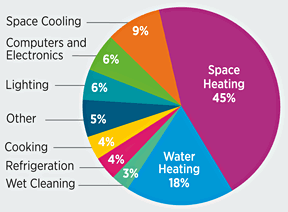
\includegraphics[width=0.35\textwidth]{1-context/images/energysaver_energyuse.png}
	\caption{An example of home energy consumption \cite{greenifynow}.}
	\label{fig:home-energy-consumption}
\end{figure}

This system will allow the user to collect and store their electricity consumption. This system will also have a web dashboard that shows the graph of electricity consumption, which the user can adjust the time range of the graph to see different data, and other useful data such as which device uses the electricity the most, etc. The data, which will be stored in our database, will be used to do analysis that will help user to predict the upcoming electricity bill in the next month and other required analysis. This system also provides a fault-tolerant computing platform to compute these analyses.

The data collection is not our part, we leave this portion of the system to the third party developers. Basically, we provide a online software service of cloud computing environment, which can be categorized as SaaS\footnote{Software as a service}, to deliver energy management system. SaaS describes when users rent or borrow online software instead of actually purchasing and installing it on their own computers \cite{whatissaas}.

Figure \ref{fig:vision} depicts the architectural vision of the HEMS.

\begin{figure}[H]
	\centering
	\includegraphics[width=0.5\textwidth]{1-context/images/vision.jpg}
	\caption{Architectural vision}
	\label{fig:vision}
\end{figure}

% \section{System Context} % (fold)
% \label{sec:system_context}
This system provides monitoring for more than one house. Many houses can connect to the system through Internet. Sensors will be located at every device that users are willing to monitor. Real time measurement of electricity consumption will be sent to the HEMS server via Internet protocol by the sensor. Users may see the energy consumption through the web dashboard via computers, tablets, smartphones, or any devices that are able to connect to the Internet.

% Figure \ref{fig:system-context} shows the system context of the HEMS.

% \begin{figure}[!ht]
% 	\centering
% 	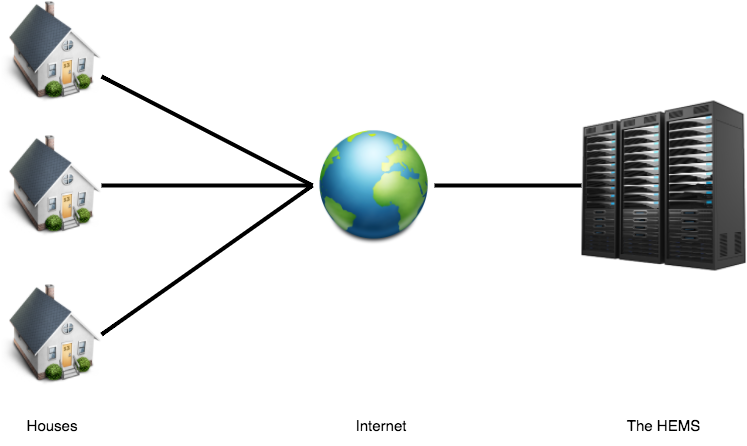
\includegraphics[width=0.7\textwidth]{1-context/images/SP-system-context.png}
% 	\caption{The HEMS system context.}
% 	\label{fig:system-context}
% \end{figure}

The rest of the document is structured as follows. The requirements, use cases, stake holders, and key drivers are explained in chapter \ref{ch:requirements}. Chapter \ref{ch:analysis} describes the analysis and lists the possible pattens to be implemented in this system. Chapter \ref{ch:system} outlines the general system architecture of the system. Hardware selection and architecture are described in chapter \ref{ch:hardware}, while chapter \ref{ch:software} elaborates on software architecture. The evaluation and evolution of this architecture is drawn in chapter \ref{ch:evaluation} and \ref{ch:evolution}. 

% %!TEX root = ../report.tex

\clearpage
\chapter{Architectural business information}
\label{ch:business}

% !TEX root = ../report.tex
\chapter{Requirements}
\label{ch:requirements}
This chapter describes our vision and uses it to derive stakeholders. This information helps us to be able to properly write use cases and stories. These will be used to extract functional, commercial, technical and evolution requirements. Afterwards, a risk assessment will take place, to ensure that the project is not at great risk.

\section{Vision}

\begin{figure}[H]
	\centering
	\includegraphics[width=0.7\textwidth]{3-requirements/images/vision.jpg}
	\caption{Architectural vision}
	\label{fig:vision}
\end{figure}

%%!TEX root = ../report.tex
\section{Architectural vision}
\label{sec:archvision}


%!TEX root = ../report.tex
\section{Stakeholders and their concerns}

%kind of QA's (accourding to "Software Requirements" 3rd edition, Karll Wiegers and Joy Beatty)
%from page 263:

This section defines all stakeholders of our system and describes the concerns of the stakeholders. A stakeholder is a person, group of persons, or organization that are involved in our system. There are ten stakeholders, ranged from first parties to third parties stakeholders. Several quality standards from the "Software Requirements" book by Microsoft \cite{wiegers2013software} are used. Those quality standards are described in \autoref{table:qa_standard}.

\begin{table}[!htbp] \centering
	\caption{Quality attributes of Software Architecture from "Software Requirements" Book \cite{wiegers2013software}.}
	\label{table:qa_standard}
	\begin{tabular}{L{\tw{0.2}} L{\tw{0.4}}}
		\toprule
		\textbf{Quality Attributes} & \textbf{Brief description}                                                                                        \\ \midrule
		Interoperability            & How easily the system can interconnect and exchange data with other systems or components                         \\
		Reliability                 & How reliable the results of the system are (accuracy). This includes availability, which is the extent to which the system's services are available when and where they are needed \\
		Security                    & How well the system protects against unauthorized access to the application and its data                          \\
		Usability                   & How easy it is for people to learn, remember, and use the system                                                  \\
		Maintainability             & How efficient and effective the system can be maintained/modified by the maintainers \\
		\bottomrule
	\end{tabular}
\end{table}

There are six quality attributes, as can be seen in \autoref{table:qa_standard}, for measuring stakeholders' concern regarding our system.  The stakeholders are listed below and are then explained in more detail below.

\begin{itemize}
%\item Product owner
\item Developers
\item Maintainers
\item Government
\item Home owners
\end{itemize}

\begin{description}

%\item [Product owner] is the owner of the system. This stakeholder funds the project.  This affects the quality attributes usability and availability.

\item [Developers] have to make sure the system provides the functionality that the users expect the system to have. They want the external components (sensors) to work with the system. This means that their main concern is interoperability, because users will want to connect any energy consuming device to this site in order to monitor the consumption.

\item [Maintainers] are mainly concerned that the website is up and running at all times. Meaning their concern is the reliability of the system. Since they are responsible for the maintenance to the system, they also care about its maintainability.

\item [The government] wants to lower the energy consumption of the citizens. It wants to comply with the aims of the EU to reduce the energy consumption by 20\% by 2020. Their main concern is that the end users will be able to use the system, so it will be widely adopted. This means they care about the usability and reliability of the system, because the system is only useful to the government if it is used by allot of people and the statistics of the system are reliable.

\item [Home owners] want to get an insight in their energy usage. They want to know how to effectively reduce their energy consumption. In order to do this, they might want to receive alerts about sudden increases of energy consumption in certain devices. These alerts have to be accurate and reliable. The main concern of the home owners, thus, is the usability of the system.

\end{description}


\autoref{table:stakeholder_concern} illustrates the stakeholder concern matrix. In our approach every stakeholder is equally important. 

\begin{table}[!htbp] \centering
	\caption{Matrix of stakeholders concern.}
	\label{table:stakeholder_concern}
	\begin{tabular}{@{} cl*{8}c @{}}
		&  & \multicolumn{6}{c}{\textbf{Concerns}} \\[2ex]
		& \textbf{Stakeholder} & \rot{Weight} & \rot{Usability} & \rot{Reliability} & \rot{Interoperability} 
		&   \rot{Maintainability} \\
		\cmidrule[1pt]{2-7}		
		 %                	      weight usa  reli  int  r main
		  %& Product owner          & 1 &     &    &     &    & & \\
		  & Developers             & 1 &     &    & 100 &     & & \\
		  %& Sensor suppliers       & 1 &   &  &  &   &    & \\
		  & Maintainers            & 1 &   & 50   &       & 50 &  \\
		  & Government             & 1 & 60  & 40 &        &&  \\
		  & Home owners            & 1 & 70  & 30  &        &&  \\
		\cmidrule{2-7}
		  & Total                  &   & 130 & 120& 100 & 50 &  \\
		\cmidrule{2-7}
	\end{tabular}
\end{table}



% !TEX root = ../report.tex
\section{Key-drivers}
The stakeholder analysis of the previous section leads to the following key drivers:
\begin{itemize}
	\item \req{kd}-- Usability
	\item \req{kd}-- Reliability
	\item \req{kd}-- Interoperability
\end{itemize}


\begin{description}

\item [Usability] has to be the main focus of the system. Users will want to stick to using our system if the usability is better then similar systems of the competitors. Even if competitors have a better availability and or even reliability, there is a good chance that customers will stick to this system if the usability is better. 

\item [Reliability] is very important, because for this kind of system the trust everyone has is crucial. Making the stakeholders trust the system is the most important aspect of this system. If the system at some points does not provide reliable data, without specifically informing about it, then the all the information from the system will be useless.
This not necessarily mean that the system has to be very precise in calculating the statistics. It just has to be very clear about how inaccurate the data is.

\item [Interoperability] is important because in order for the system to be useful to the user, it has to collect and process the energy consumption of devices. All the different homes have different devices who each have a different set of relevant statistics to be calculated.
The sensor data will be monitored with a energy monitoring plug. However, to be able to receive valuable statistics from this data, the system needs to be able to cope with different types of devices.
%
%if the system isn't up at the times when it should, users will lose trust in the system. If a user set an alarm on a device, alarming them if the device exceeds a certain energy consumption, then ideally that alarm has to go any time the device indeed exceeds the given limit of energy consumption.

\end{description}

%!TEX root = ../report.tex

\clearpage
\section{High-level requirements}
The high-level requirements describe the high-level functionality of the system. The high-level requirements are used to derive the functional requirements in section~\ref{sec:functional-requirements}. The high-level requirements are also used to classify the severity of the risks in section~\ref{sec:risk-assesment}. 

This table uses different priorities. First there is the `must' priority, this requirement is an absolute must. The system could not function without the `must' requirement. Besides `must' there is the `should' priority. This priority is highly desirable for the system, but the system could function without this requirement. The last priority is `could', these requirements are nice to have but not really necessary for the core functionality of the system. These different priorities are used through the rest of the document.

\begin{longtable}{L{0.1\textwidth} L{0.12\textwidth} L{0.78\textwidth}}
	\textbf{Nr.} & \textbf{Prio} & \textbf{Description} \\
		
	\hlReqRow{collecting}{Must}{Collecting electricity usage data}
	{ The system must collect electricity usage data, which has to be stored so it can be used to compute statistics and detect changes in energy usage. }
	
	\hlReqRow{analyzing}{Must}{Computing usage statistics}
	{ The system must be capable of computing statistics about the energy usage, like total usage per month, but also periods of peak energy usage. It has to be able to compute such statistics not only per house, but also for individual devices. }
	
	\hlReqRow{analyzing}{Must}{Displaying usage data / statistics}
	{ Data which has been gathered and statistics that have been computed must be displayed to the user in an understandable way. One of the main goals of the system is to make users of the system aware about their energy usage. The data and statistics should be displayed in a way that is intuitive and easy to understand for average consumers. }
	
	\hlReqRow{configuration}{Must}{Configuring the system}
	{ The users of the system must be able to configure the system, i.e. register their house/add new devices/subscribe to alerts etc., using the web interface. This web interface should be user-friendly and intuitive, such that an average consumer is able to use it. }
			    
	\bottomrule

\caption{High Level Requirements}
\label{table:high-level-requirements}	    
\end{longtable}


%!TEX root = ../report.tex
\clearpage
\section{Stories and use-cases}

In this section the architectural significant ue-cae will be presented.

% Installation ?
% Collect and store energy consumption
% The End-Uer wants to display his bill ( to specific ? ) / his energy conumption
% Update ?
% Computation ? by Spark , Map/Reduce , DOES THE SYSTEM COMPUTE THE STATISTICS ONLY WHEN THE USER ASKS FOR PECIFIC STATITICS OR EVERYTIME ?



\textbf{The End user registration} \\
\textit{Number} : UC-1 \\
\textit{Goal} : The user has to register on the website to create his account.
\textit{Primary Actor }:  End-User \\
\textit{Precondition}: The website has the internal process to add an user to the database
\textit{Main Success Scenario }: \\
 1. The user acess the HEMS URL \\
 2. The user click on the " Sign up " Button \\
 3. The website display a regitration form requests the Fullname, Username, email adress and adress of the user.\\
 4. The system checks if the user isn't already in the database. \\
 5. If not the user is added in the database. \\
 6. The user receives a confirmation link on his email adress and clicks on it. \\ % or verification code ?
 7. The user is redirected to the HEMS webite. \\
\textit{Extensions} 1. The user isn't added to the system database. \\
1a. An error message is displayed " The regitration failed, do you want to try again Y/N? ".
1a. If yes Go to step 3.
%2. The user is already in the database.
\textit{Postcondition} : The account is created : the user get acces to his own Home Energy Monitor interface. \\

\textbf{Receive / Collect external energy data} \\% (out of scope ?) \\
\textit{Number}: UC-2 \\
\textit{Goal}: The sytem needs to receive energy data to make the analysis. \\
\textit{Primary Actor} : The system \\
\textit{Precondition}: The energy data is available. \\
\textit{Main Success Scenario}: \\ % what is the process ?
\textit{Extensions} \\
\textit{Post condition}: \\

\textbf{Store energy consumption}\\
\textit{Number} : UC-3 \\
\textit{Goal}: The system needs to store the energy data it just received. \\
\textit{Primary Actor}: System \\
\textit{Precondition} : 1. The system can receive the data. \\
2.The sytem has a database \\
\textit{Main Success Scenario} : 1. The data received is directly stored in the database. \\
\textit{Extensions} : The data isn't stored. % why ? \\
\textit{Post-condition}: The data is in the database.\\

\textbf{Display the next bill}\\
\textit{Number} : UC-4 \\
\textit{Goal}: The End-Uer wants to display the estimation of his next bill \\ 
\textit{Primary Actor}:  End-User \\
\textit{Pre-condition}: The user is registered in the database of the system.\\
\textit{Main Success scenario} : \\
1. The user gets acess to his interface by clicking on "Sign in" Button\\ % sign up ?
2. In the menu he clicks on the "Bill" button.\\
3. In the bill section the user chooses the "Next bill". \\ % the previous ones are alo available
\textit{Extensions} \\
% Authentification failed
\textit{Postcondition} : The bill is displayed.

\textbf{Display analysis, daily/weekly/monthly report}\\ % too generic ?
\textit{Number} : UC-5 \\
\textit{Goal}: The End-Uer wants to display several kind of analysis about hi energy consumption \\ 
\textit{Primary Actor}: End-User \\
\textit{Pre-condition}: The user is registered in the system.
\textit{Main Success scenario} : \\
1. The user gets acess to his interface by clicking on " Sign in " Button \\
2. In the menu he clicks on " Analyis- Chart " \\ 
3. The system computes/make the analysis. \\
\textit{Extensions} : The statistics aren't made. \\
\textit{Postcondition} : Charts with different item are displayed.

\textbf{Update}\\
\textit{Number}: UC-6 \\
\textit{Goal}: The sytem needs to update itself. \\
\textit{Primary Actor} : The system \\
\textit{Precondition}: \\
\textit{Main Success Scenario}: \\
\textit{Extensions} \\
\textit{Post condition}: \\

\textbf{Configuration} \\
\textit{Number}: UC-7\\
\textit{Goal}: The user must be able to configure the sytem with his own characteritics. \\
\textit{Primary Actor} : The user \\
\textit{Precondition}: The user is registered in the database of the system. \\
\textit{Main Success Scenario}: 1. On the dashboard/website the user clicks on the " Settings " button. \\
2. The user gets access to the Settings section with all the possibilities/internal sections for example :frequency of alert, adding new devices etc.\\
\textit{Extensions}:1. The system didn't take into account the information the user just added. \\
1a. An error mesage is displayed " Configuration failed, would you like to try again Y/N ? ". \\
If yes Go to step1. \\
\textit{Post condition}:The system is set with the user's characteritics of his home and preferences. \\

%!TEX root = ../report.tex
\newpage
\section{Functional requirements}
\label{sec:functional-requirements}

% !TEX root = ../report.tex
\section{Technical non-functional requirements}
In this section, the technical non-functional aspects that are important to the system are described.

\subsection{Usability}
The sytem will be hopefully used by a lot of people who don't necessarily have knowledge in the technology field so the Usability is an important requirement so the end-user can acces all the information he needs. \\

 	\pgfplotstabletypeset[%
 		UCTable
 	]{%
 		value & description \\
 		\req{US} & An application is available for tablets and phone with those OS Windows Phone,Android, and Iphone. \\
 		\req{US} & The end-user needs maximum ten minutes to get a basic understanding of system features through the UI. \\
 		\req{US} & Every feature/major option of the system can be accessed through the home page(Single Page Application). \\
 	}

% Email The user can receive an email with the information he aked (for example etimate bill) once a month.
%Error message

\subsection{Reliability}
 	\pgfplotstabletypeset[%
 		UCTable
 	]{%
 		value & description \\
 		\req{RE} & A margin of error of $5\%$ in the energy measurements is tolerated. \\
 		\req{RE} & The sytem should be available $99.9\%$. of the time which means down for 44 minutes. \\
 		\req{RE} & The system should be down for maximum ten minutes when the user installs a new release(version). \\
 	}
%$AV = \frac{\text{MTTF}}{\text{MTTF} + \text{MTTR}} = \frac{\text{6 months}}{\text{6 months }+\text{ 12 hours}} = \frac{4380 \text{ hours}}{4380 + 12 \text{ hours}} = 99.7 \%$
% computation
 	
\subsection{Security}
Ensuring the security for the system is a major issue so all the data needed for its good functioning remain protected and consistent. \\

 	\pgfplotstabletypeset[%
 		UCTable
 	]{%
 		value & description \\
 		\req{SEC} & Each user is identified and has to log in in order to view his "Home Energy Monitor" account. \\
 		\req{SEC} & The data is encrypted. \\ % developp , which database ?
 	}

\subsection{Interoperability}
\pgfplotstabletypeset[%
 		UCTable
 	]{%
 		value & description \\
 		\req{INT} & The web interface of the system is available and functioning for 95\% of the browser market share. \\
 		\req{INT} & The system exposes a REST interface that allows different electricity usage sensors to submit the electricity usage data. \\ 
 	}
 

\subsection{Scalability} 
The system should make the increase of workload, resources and users easy.\\
 	\pgfplotstabletypeset[%
 		UCTable
 	]{%
 		value & description \\
 		%\req{SCA} & The system must be able to monitor several kind of energy consumption for example: gas ,solar, temperature. \\
 	\req{SCA} & The system should function as efficiently even if the number of users increases. \\% increase in the number of users \\
 	}

%!TEX root = ../report.tex
%\section{Evolution requirements}
%\label{sec:evolution-requirements}

%!TEX root = ../report.tex
\newpage
\section{Risk assessment}
\label{sec:risk-assesment}

The system is confronted by several risks which are determined and mitigated in this section.
Taking those risks into account allows to avoid them or at least reduce their impact. 
The risk management involves the identification of the risks, their probability and potential impact or consequences.

The tables below explain the meaning of the definition for probability and consequence.
\begin{figure}[H]
	\centering
	\begin{tabular}{|c|c|}
		\hline \textbf{Probability} & \textbf{Likelihood of occurrence} \\ 
		\hline High                 & 0.65 - 1.00                       \\ 
		\hline Medium               & 0.35 - 0.65                       \\ 
		\hline Low                  & 0.00 - 0.35                       \\ 
		\hline
	\end{tabular} 
	\caption{The different probabilities used to classify risks}
	\label{table:risk-probability}
\end{figure}

\begin{figure}[H]
	\centering
	\begin{tabular}{|l|p{15.5cm}|}
		\hline \textbf{Severity} & \textbf{Explanation}                                                                                                                        \\ 
		\hline Severe            & A risk that can lead to loss of live or casualties.                                                                                         \\ 
		\hline Significant       & A risk that can lead to damages, can delay the project more than 3 months or causes one of the high-level requirements not to be fulfilled. \\ 
		\hline Moderate          & A risk that can lead to one of the high-level requirements not to be fulfilled to an acceptable level.                                      \\ 
		\hline Minor             & A risk that can lead to one of the high-level requirements not being fully fulfilled, but still fulfilled in an acceptable level.           \\
		\hline
	\end{tabular} 
	\caption{The different severities used to classify risks}
	\label{table:risk-severity}
\end{figure}


\subsection{Technical}
%\risk{T}
%{The energy measurements provided by the data center are wrong.} 
%{Low}
%{}
%{}
%{}
%{risk:wrong-measurement}
 % AF: who provides the data ? 
 %  WM: i think the devices in the house provide the data

\risk{T}
{The statistics provided by the data processing framework are wrong}
{Low}
{Moderate. If the statistics computed by the system are not accurate, this will lead to loss of thrust of the end user in the system.}
{Make sure the algorithms used to compute the statistics are correct.}
{Correct the algorithm, if the change is significant also inform end users about the error.}
{risk:wrong-statistics}

\risk{T}
{The data center storing the energy measurements becomes unavailable}
{Low}
{Significant}
{Store the data in a redundant way, preferably in multiple data centers, so that one data center going offline does not lead to downtime of the system.}
{If the data storage does become unavailable, new incoming data should be cached so it is not lost and users should be informed in the web interface that viewing the statistics is temporarily unavailable.}
{risk:unavailability}

\risk{T}
{Somebody gains unauthorized access to someone else's data}
{Low}
{Significant. Data about electricity usage can be used, e.g. to derive when people are home. Unauthorized data access will lead to a loss of thrust in the system by consumers.}
{Make sure access to the data requires authentication using a password at all time. Enforce users to use a strong password.}
{Make sure the unauthorized access is removed. Inform end users about which data was accessed by the unauthorized party.}
{risk:unauthorized-access}

\subsection{Business}
\risk{B}
{Wrong estimation of the budget}
{Medium}
{Significant. The final product does not have the features expected.}
{The team needs an accountant or at least someone taking care of the follow-up of the money. Make sure there are regular evaluations to keep track of the money flow.}
{Remove some requirements or features of the product, or change the hardware components used.}
{risk:budget}

\risk{B}
{Wrong estimation of the budget: the money invested in the fabrication and achievement of the product/system is not covered by the sales (shortfall/deficit)}
{Medium}
{Moderate. Stopping the sale}
{The team needs an accountant or at least someone taking care of the follow-up of the money.}
{Adding more features to the product in order to make it more competitive in the market.}
{risk:shortfall}

\subsection{Schedule}


\risk{S}
{The project is not finished at the deadline}
{Low}
{Significant. Pressure for all the team members, loss of credibility regarding the customers, selling a product with less features than expected.}
{ SRA , Schedule Risk analysis : Estimation of the duration of the project by its manager ( with the use of probability and statistics ) . Meeting for the team members every week to keep track of the timing and take decisions according to the deadline. }
{ Postpone the deadline or remove some features when the deadline can't be postponed. }
{risk:schedule}


% !TEX root = ../report.tex
\chapter{Analysis}
\label{ch:analysis}

%All layers (with their patterns) is very clearly described in ch8 starting on p95.

\newcommand{\EAA}{Patterns of Enterprise Application Architecture}

%\section{Layers}
%
%\begin{description}
%%
%%Context – a recurring set of situations in which the
%%pattern applies.
%%Problem - a set of forces (goals and constraints)
%%occurring in this context.
%%• Forces are often competing
%%Solution - a canonical design form or rule that
%%someone can apply to resolve these forces.
%%• The solution balances the forces.
%
%\item [Context]
%
%
%\item [Problem]
%The system needs a structure to coordinate the external calls and requests.
%
%\item [Solution]
%Our application exposes a web service to multiple clients and so a the Service Layer pattern will be used. Using this pattern, the system will be divided into the following layers.
%
%
%
%\item [Source] 
%\EAA  \cite{Fowler:2002:PEA:579257}
%\end{description}

\section{Layers}
\manuallabel{sec:layers}{Layers}

\begin{description}
\item [Source]~\\
Pattern-oriented Software Architecture - Volume 1 \cite{wiley-1}

\item [Issue]~\\
The system consists of high-level components (e.g. user interface), which are dependent on lower level components (domain logic, database). Decoupling these components is important.

\item [Assumptions/Constraints]~
\begin{itemize}
\item It is assumed that the system will have higher-level components that depend on lower-level components.
\end{itemize}
~\\[-1.5cm]

\item [Positions]~
\begin{enumerate}
\item Relaxed Layered System
\item Layers
% Indirection Layers??
\end{enumerate}
~\\[-1.5cm]

\item [Decision] ~\\
The system will use the Layers pattern to divide the application in multiple layers. The top layer will implement the Service Layer pattern, the middle layer will implement the domain logic (domain model) and the bottom layer will be responsible for the data storage.

\item [Argument]~
\begin{enumerate}
\item The relaxed layered system is a variant of the Layers pattern which allows layers to use services of any layer below it, instead of only the next layer. This increases the flexibility and performance of the system. However, this pattern has a large negative impact on the maintainability.

\item 
Using the layers pattern increases maintainability by decoupling components of different levels of abstraction.

\end{enumerate}

\item [Implications]~\\
Using layers will have a positive impact on the maintainability and re-usability of the system. An increased maintainability will help prevent bugs, which on the longer term helps to increase the reliability of the system. 

The performance of the system will have some negative impact, since the request have to pass all the layers, even if they only need logic/data in the bottom layer.

\item [Related requirements/decisions]~\\
\ref{sec:service-layer}, 

\end{description}


\section{Service Layer}
\manuallabel{sec:service-layer}{Service Layer}

\begin{description}
\item [Source]~\\
Patterns of Enterprise Application Architecture, P.133 \cite{Fowler:2002:PEA:579257}

\item [Issue]~\\
The system will have different interfaces with different kinds of clients. For example, commands to compute statistics can come from the user interface, but also from the alerting module. These different interfaces have common interactions with the system to invoke the business logic. %TODO describe altering module in elaborated model

\item [Assumptions/Constraints]~
\begin{itemize}
\item The application's business logic and/or data are accessed using several interfaces.
\end{itemize}

\item [Positions]~
\begin{enumerate}
\item Domain Model % just domain model not good enough
\item Service Layer
\end{enumerate}
~\\[-1.5cm]

\item [Decision] ~\\
The system will use the Service Layer pattern to define the boundary of the application using a layer of services.

The service layer exposes a set of services to be used by clients and for each service, there is a certain script that will be executed when the service is called. The service layer will be used with the "operation script" variation. This means that the Service Layer consists of thick classes that contain logic. %TODO Why do we want thick classes with logic?????

\item [Argument]~
\begin{enumerate}
\item Using just the Domain Model pattern alone does not make a distinction between application logic and domain logic.

\item The service layer does allow making a distinction between the application- and domain logic, which 
\end{enumerate}

\item [Implications]~\\
There is a boundary between the application- and domain logic.

\item [Related requirements/decisions]~\\
\ref{sec:layers}, \ref{fr:interface-selectstats}, \ref{fr:receive-usage}

\begin{figure}[H]
\caption{Service Layer}
\centering
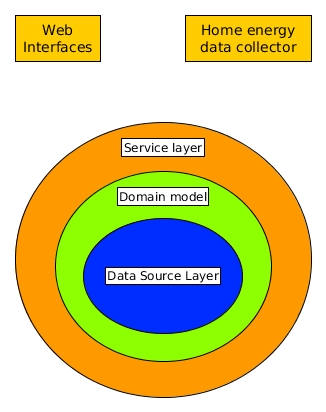
\includegraphics[scale=0.7]{4-analysis/images/ServiceLayer.jpg}
\end{figure}


\end{description}


%\section{Layer Supertype}
%
%\begin{description}
%%
%%Context – a recurring set of situations in which the
%%pattern applies.
%%Problem - a set of forces (goals and constraints)
%%occurring in this context.
%%• Forces are often competing
%%Solution - a canonical design form or rule that
%%someone can apply to resolve these forces.
%%• The solution balances the forces.
%
%%\begin{description}
%%\item [Context]
%%\item [Problem]
%%\item [Solution]
%%\item [Source]
%
%\item [Context]
%There is duplicate code within each layer of the system.
%
%\item [Problem]
%Duplicate code makes the system hard to modify and maintain.
%
%\item [Solution]
%With the Layer Supertype pattern, all the classes of a certain layer have the same super class. This super class then contains the features that are very common for the layer.
%
%This pattern will be used in every layer.
%\begin{description}
%\item[Service layer] All the services need to take care of security. The client needs to be authenticated and the data needs to be decryption by the service layer. All this security logic will be placed in a super type using the "Layer Supertype" pattern In the service layer it contains the security logic.
%
%\item[Domain layer] In this layer, the sypertype will contain common features and functions for handling storage.
%%\myworries{From book:
%%-  "Common features, such as the storage and handling of 'Identity Fields (216), can go there."}
%
%\item[Data source layer]
%The data mapper in the data source pattern can use a layer super type that handles all the common behavior, which can greatly reduce the extra work of coding. 
%
%%(p308 (Metadata mapping pattern))
%\end{description}
%
%%\myworries{p475 POEAA
%%"A type that acts as the super type for all types in the layer".}
%
%\end{description}

\section{Domain layer}

\begin{description}
\item [Context]
The domain logic consists of complex functions for serving web request and analyzing data.

\item [Problem]
The functionality of the system must be modifiable and must not contain duplicate code to prevent inconsistency.

\item [Solution]
The domain logic is complex and so it requires the use of the domain model pattern. This means that the domain is Object Oriented, with every class representing one specific, individual, meaningful part.
This is the most advanced pattern, reducing code duplication and increasing flexibility of the system.

%The alternatives are : Transaction Script and Table module.
%
%Transaction script: Each system call has its corresponding script that will be executed.\\
%Table module: One class per table in the database that contains all the logic acting on that data.

\item [Source]

\end{description}

\section{Unit of work}

\begin{description}
\item [Source]~\\
Patterns of Enterprise Application Architecture, P.184 \cite{Fowler:2002:PEA:579257}

\item [Issue]~\\
The system has several object stored in a database which can be edited and created. For example, new sensor data of devices becomes available and changes to the configuration (changing device names etc.) can be made. Updating database records on each change leads to a lot of database calls, which is bad for performance.

\item [Assumptions/Constraints]~\\

\item [Positions]
\begin{enumerate}
\item Active Record
\end{enumerate}

\item [Decision] ~\\
Unit of Work pattern will be used to keep track of changes to objects and to coordinate writing these changes to the database in one database call.

\item [Argument]~\\
With Active Record, every change to an in-memory object leads to a database call. This means that multiple consecutive changes to an object lead to multiple database calls. 

The Unit of Work instead keeps track of these changes, to allow writing these changes to the database in a single call.

\item [Implications]~\\
Using Unit of Work will reduce the load on the database (the number of database calls). It does however introduce a delay before the change in the in-memory object is present in the representation in the database.

\item [Related requirements/decisions]~\\
--

\end{description}

\section{Broker}

\begin{description}
\item [Source]~\\
Pattern-oriented Software Architecture - Volume 4 \cite{wiley-4}

\item [Issue]~\\
The system uses several servers to compute the statistics. This introduces a lot of challenges, like communication to these servers and dividing the work over these servers. The application code should not have to address these challenges.

\item [Assumptions/Constraints]~\\

\item [Positions]~
\begin{enumerate}
\item Publisher-Subscriber
\item Broker
\item Message Queuing
\item Remote Procedure Call
\end{enumerate}
~\\[-1.5cm]

\item [Decision] ~\\


\item [Argument]~\\


\item [Implications]~\\


\item [Related requirements/decisions]~\\
\ref{fr:compute-total}, \ref{fr:compute-bill}, \ref{fr:compute-bill}
%Refer to layers
%Most B ROKER realizations are based on a L AYERS (185) architecture
%to manage complexity, such as CORBA [OMG04a] and Microsoft’s
%.NET Remoting [Ram02]. These layers are further decomposed into
%‘special-purpose’ components for specific networking and communi-
%cation tasks. We illustrate this partitioning using the CORBA layering
%[SC99]—other layering schemes and middleware may involve differ-
%ent assignments [VKZ04].

\end{description}


\section{Data source layer}
The main database will be quite simple and the database actions won't be very complicated. However, the tables needed for the statistics can become very complex.

\begin{figure}[H]
\caption{Database structure draft}
\centering
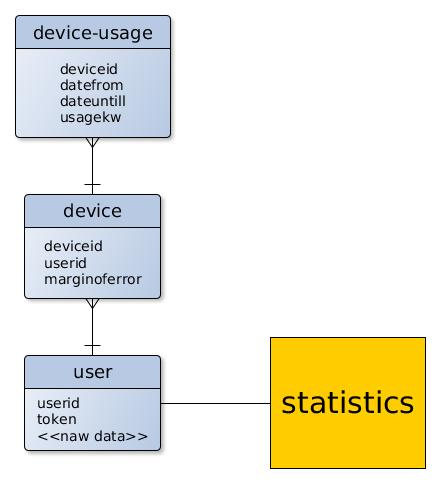
\includegraphics[height=10cm]{4-analysis/images/SoftwarePatternsDatabaseDraft.jpg}
\end{figure}

Considered patterns to connect to data sources:
\begin{itemize}
\item Table data gateway% (p144)
\item Row data gateway% (p152)
\item Active record %(p160)
\item Data mapper% (p165)
\end{itemize}

Because the domain model is used in the domain layer, the data mapper pattern is best to use . \ign{(153 and 97)}
The logic that will operate on the data will generate statistics of the data, which can become quite complex. This is why the data mapper pattern is chosen as a pattern for connecting to the data sources. This pattern is the most advanced pattern, but provides the best functionality and abstraction.

With the active record pattern, the database access/communication, data and logic of that data is all stored in the same class. Since the logic that will be executed on the sensor data is very complex, this patterns will not be useful.

A gateway of any kind leads to performance overhead, because for each call coming from the domain model pattern, a database call is made. It lacks the necessary coordination.
%
%\subsection{Table data gateway}
%\myworries{Not needed if the repository is used (i assume)}
%
%The data mapper can use the table data gateway to remove the dependency on how the data is queried. Queries can be replaced with stored procedures in the Table data gateway without the data mappers having to change 
%
%%Using a record set (504) turning into a unit of work (184)? P98 (lost the page:()

\subsection{Repository}
%\myworries{
%P322:
%"Mediates between the domain and data mapping layers using a collection-like interface for accesing domain objects."
%\\
%P323:
%"Repository supports the objective of achieving a clean separation and one-way dependency between the domain and data mapping layers"
%\\
%P324:
%"Under the covers, Repository combines Metadata Mapping (329) with a Query object (316) to automatically generate SQL code from the criteria."
%...
%"In a large system with many domain object types and many possible queries, Repository reduces the amount of code needed to deal with all the querying that go's on."
%}

The repository pattern mediates between the domain and data layer. The repository clients create a criteria object, specifying what kind of data is wanted. For example $criteria.equals(Device.NAME, Computer)$. Then the clients use this criteria by invoking repository.matching(criteria) to receive the data from the repository. The client just asks the data, it has no further knowledge about any interaction with any data source/data base.

The repository gives a lot more control over how the data is handled. The benefits are:
\begin{itemize}
\item Reduces code (and code complexity)
\item Increases performance
\item Separated domain and data layers, increasing flexibility and changeability
\end{itemize}

Performing analysis on the data also consists of executing complex queries on the data source. The database that executes these queries, however, might change. Or the system might decide to use multiple databases and data sources.
Using the Repository pattern, these changes can be made fast. The repository also allows for multiple configurations to exist. So an extra repository could be created for testing purposes, only using an in-memory database to increase the test execution speed.

% \section{Client user interface}

% \subsection{Controller}
% %\myworries{
% %On p 99:
% %\begin{itemize}
% %\item Given a free choice, I'd recommend Page Controller (p333). 
% %\item More complex navigation and UI lead you toward a Front Controller (344)
% %\end{itemize}
% %}
% Page controller: controller for each page. So upon receiving a request do:
% \begin{itemize}
% \item decode url, extract data
% \item invoke model to process data
% \item determine view and use the model data to create the HTML to return
% \end{itemize}

% Front page controller:\\
% One controller for all requests/views. This allows building a filter chain, handling authentication, logging etc.
% Front page is better/helps with concurrency, because a new command object is created on each request. Reducing thread-safety concerns. \ign{(P346)}The model, however, can have shared objects that do require thread safety management.

% The front page will be used, because it provides more functionality to the system. The only advantage of a page controller compared to the front controller is that it has a more natural structure.

% \subsection{View}
% %\myworries{
% %Template view (350) or Transform view (361).
% %\\
% %(P forgot):
% %Template views have the edge at the moment.
% %}

% \begin{description}
% \item [Template view] Write HTML code including markers. Replace the markers with the data when the page is requested. (Play framework)
% \item [Transform view] Convert the domain data to HTML, "transform" the domain data. Upon a request, it get the domain data, for each item in the data it looks for a appropriate "transform" to transform the data to HTML.
% \end{description}

% The template view will be used, because it is used a lot more then the transform view. Major web frameworks are based on this pattern (the play framework, laravel...). The view patterns don't have an important difference in how beneficial they are to the project.

% %Transform view avoids having too much data in the HTML, because of the transform methods creating the HTML.
% %Transform view can be tested without having a web server up.

% \subsection{Model}
% %\myworries{
% %Communication with the model: p100:
% %Preference: Having everything run in one process if you can. Else Remote Facade (p388) and DTO (p 401).
% %}
% %
% %\myworries{
% %\section{Notes only}
% %\subsection{Model-View View-Model}
% %}
% This section will describe how the Model updates the view and how the view updates the model.
% %\myworries{View update model using page controller as is already described}

% To consider:
% \begin{description}
% \item [Observer Synchronization] Synchronize multiple screens by having them all be observers to a shared area of domain data.
% \item [Separated Presentation] Ensure that any code that manipulates presentation only manipulates presentation, pushing all domain and data source logic into clearly separated areas of the program.

% \item [Presentation model] Represent the state and behavior of the presentation independently of the GUI controls used in the interface

% \item [Supervising controller] Factor the UI into a view and controller where the view handles simple mapping to the underlying model and the the controller handles input response and complex view logic.

% \item [Model view controller/presenter] 

% \end{description}

%Observer Synchronization
%%Synchronize multiple screens by having them all be observers to a shared area of domain data.
%%\url{http://www.martinfowler.com/eaaDev/uiArchs.html}
%%While Observer Synchronization is nice it does have a downside. The problem with Observer Synchronization is the core problem of the observer pattern itself - you can't tell what is happening by reading the code. I was reminded of this very forcefully when trying to figure out how some Smalltalk 80 screens worked. I could get so far by reading the code, but once the observer mechanism kicked in the only way I could see what was going on was via a debugger and trace statements. Observer behavior is hard to understand and debug because it's implicit behavior.
%
%Separated Presentation:
%%\url{http://martinfowler.com/eaaDev/SeparatedPresentation.html}
%Ensure that any code that manipulates presentation only manipulates presentation, pushing all domain and data source logic into clearly separated areas of the program.
%%Most of examples you'll see from me follow Separated Presentation, simply because I find it such a fundamental design technique
%
%Presentation model:
%%\url{http://www.martinfowler.com/eaaDev/PresentationModel.html}
%Represent the state and behavior of the presentation independently of the GUI controls used in the interface
%
%Supervising controller\\
%Factor the UI into a view and controller where the view handles simple mapping to the underlying model and the the controller handles input response and complex view logic.
%
%%MVP potel:
%%\url{Potel: http://www.wildcrest.com/Potel/Portfolio/mvp.pdf}

\section{Model-View-Controller}
\begin{description}
\item [Source]~\\
Pattern-oriented Software Architecture - Volume 1 P.125 \cite{wiley-1}\\
Patterns of Enterprise Application Architecture, P.330 \cite{Fowler:2002:PEA:579257}

\item [Issue]~\\
The system must handle the request from user by dynamic web interface. In order to increase re-usability, the views may be decoupled from the logic, resulting in separated logic (controller and model) and view.

\item [Assumptions/Constraints]~
\begin{itemize}
\item It is assumed that the client uses web browser to connect to the system.
\item It is assumed that there are multiple views in the system.
\end{itemize}
~\\[-1.5cm]

\item [Positions]~
\begin{enumerate}
\item Presentation-Abstraction-Control
\item Layers-Model-View-Controller
\end{enumerate}
~\\[-1.5cm]

\item [Decision] ~\\
The system will use the Model-View-Controller pattern to decouple the view and the logic behind it. This pattern resides in the service layers of this system.

\item [Argument]~
\begin{enumerate}
\item The Presentation-Abstraction-Control (PAC) pattern decompose the system into a tree-like hierarchy of agents, which each agent is made of its own presentation (UI), abstraction, and control. This type of pattern is not well suited to the HEMS since the HEMS only needs decoupled views with the same control and abstraction.

\item The Model-View-Controller (MVC) pattern only decouple the views, models, and controller, which indicates that different views may use the same controller and/or model. This pattern is well-suited with the HEMS and is good for re-usability, which we think has less complexity.

\end{enumerate}

\item [Implications]~\\
By implementing the MVC pattern, several views are created to support multiple pages. Each view may use the same controller that provides required process. This will also allows building a filter chain, handling authentication, logging etc. Thus, this will drive better reusability and have less complexity. Furthermore, it is also easier to modify the code since the view and the logic are separated.

\item [Related requirements/decisions]~\\
\ref{fr:retrieve-usage}, \ref{fr:interface-selectstats}, \ref{fr:interface-login}, \ref{fr:alerts}, \ref{fr:interface-graph} 

\end{description}



\section{Template view}
\begin{description}
\item [Source]~\\
Patterns of Enterprise Application Architecture, P.350 \cite{Fowler:2002:PEA:579257}

\item [Issue]~\\
In the view component of MVC, the system must handle dynamic web interface in a Single Page Application (SPA) flavored application. The same view (HTML code) will be displayed several time in different page, which will be possibly causing code smells.

\item [Assumptions/Constraints]~
\begin{itemize}
\item This pattern is only applied on web application.
\item The system is developed using framework that supports this pattern.
\end{itemize}
~\\[-1.5cm]

\item [Positions]~
\begin{enumerate}
\item Transform view
\item Two step view
\item Template view
\end{enumerate}
~\\[-1.5cm]

\item [Decision] ~\\
The system will utilize template view in order to increase reusability and to prevent code smells in the project. In this way, several HTML code snippets that corresponds to same element of a page will be reused by embedding markers. Thus, this will lead to a better modifiability as well.

\item [Argument]~
\begin{enumerate}
\item Transform view processes domain data element by element and transforms it into HTML. In the system, such task is handled by the models. Thus, if this pattern is used, there will be duplication of work.

\item Two step view turns domain data into HTML in two steps: first by forming some kind of logical page, then rendering the logical page into HTML. These operations are considered as inefficient, as the forming logical page and rendering HTML can be joined. There is also overlapping between models, controllers, and views in this pattern.

\item Template view renders information into HTML by embedding markers in an HTML page, which solves the issues and prevents code smells.
\end{enumerate}

\item [Implications]~\\
Several HTML code snippet will be reusable, which is good for reusability and simplicity. Furthermore, code smells can be prevented using this template view.

\item [Related requirements/decisions]~\\
\ref{fr:retrieve-usage}, \ref{fr:interface-selectstats}, \ref{fr:interface-login}, \ref{fr:alerts}, \ref{fr:interface-graph}

\end{description}


%!TEX root = ../report.tex
\chapter{System architecture}
\label{ch:system}

% !TEX root = ../report.tex
\section{System context}
\label{sec:system-context}

The system context diagram in Figure~\ref{fig:system-context-diagram} gives an overview of the entities that interact with the system.

\begin{figure}[H]
	\centering
	\includegraphics[keepaspectratio=true,scale=0.5]{5-system/images/SystemContext.png}
	\caption{System context diagram}
	\label{fig:system-context-diagram}
\end{figure}

\subsection{Users and roles}
\begin{description}

	\item[Home Owners] ~\\ The home owners are the main users of the system. They want to know about the electricity usage in their house. 
	
	They interact with the system by viewing statistics, configuring the system and they receive alerts if they configured the web interface to send these. 
	
	\item[Maintainers] ~\\ The maintainers of the system will apply updates to the system and read errors that might have occurred in order to solve these.
	
\end{description}

\subsection{External systems}
\begin{description}

	\item[Electricity Usage Sensors] ~\\ The electricity usage sensors are the sensors that measure the electricity usage of the devices. These sensors work by measuring the electricity passing through a power outlet. This means that they in fact measure the electricity usage of a power outlet and not that of a device. This is relevant if multiple devices are connected to the same power outlet .
	
	\item[Web Browsers] ~\\ The web interface of the system, where the system can be configured and statistics can be viewed, is presented as a web page. Users will use a range of different web browsers (on a range of different devices) to visit this web interface. It is important that the web interface works equally well in all these different web browser.
	
\end{description}


%!TEX root = ../report.tex
\section{Verification}

% !TEX root = ../report.tex
\section{Elaborated Model}
\label{sec:elaboratedmodel}

In Figure~\ref{fig:elaboratedmodel} the elaborated system model is shown. This figure gives a high-level overview of the software and hardware of the system. In this figure, the arrows represent the data flow.

Each house sends collected electricity usage data to the systems `Data receival API', which stores the collected data in a storage cluster.
An end-user of the system can visit the web interface using a web browser on any device. Using this web interface, the user can generate statistics data, which is done by a separate software component of the system.

%TODO: update diagram for configuration/registering new devices etc.

\begin{figure}[H]
	\centering
	\includegraphics[keepaspectratio=true,scale=0.45]{5-system/images/HighLevelOverview.png}
	\caption{Elaborated model}
	\label{fig:elaboratedmodel}
\end{figure}

\begin{description}
	\item[Data receival API] ~\\ The `Data receival API' component exposes a REST interface, which is used by the homes to send electricity usage data to the system. The API is responsible for storing the data in the storage cluster or caching the data if the storage cluster is temporarily not available.
	
	\item[Storage cluster] ~\\ The storage cluster is a set of servers which will store all the data in a replicated way.
	
	\item[Web interface] ~\\ Users of the system (home owners) visit the web interface (presented as a website) through all kinds of devices. The web interface allows users to compute and view statistics from the collected usage data. The web interface also allows users to register new devices with the system.
	
	\item[Statistics] ~\\ The statistics part of the system is responsible for computing statistics from the collected usage data. It will receive commands to do so through the web interface.
	
	\item[Compute cluster] ~\\ The compute cluster is a cluster of servers, which are used to compute statistics from the raw collected electricity usage data.
	
\end{description}


%!TEX root = ../report.tex
\chapter{Hardware Architecture}
\label{ch:hardware}
This section describes the hardware architecture of Home Energy Management System (HEMS). The description will be more high-level along with explanations about the hardware platform and the application interfaces between each components of the system. The rest of this chapter is organized as follows; First section, \autoref{sec:hardware-overview}, presents an overview of the hardware implemented in this system depicted in big schema. Decisions made in this system are detailed in \autoref{sec:hardware-decisions} with tables. Lastly, the hardware is described in \autoref{sec:hardware-description}.

%!TEX root = ../report.tex
\section{Hardware Overview}
\label{sec:hardware-overview}
As mentioned in previous chapters, HEMS focuses on providing services to monitor electricity usages based on installed sensors on each customer's house. Thus, this system works on the cloud part, which is providing data storage, monitoring, and analysis, both in terms of application (software or service) and hardware. This system deals with no electricity collecting devices. Therefore, the electricity collection part is delegated to third party developers.

According to chapter system architecture, the main part of the HEMS hardware consists of storage cluster and compute cluster. The storage cluster is responsible to handle incoming data from sensors through the exposed data acquisition API. This cluster is capable to store real-time data. The compute cluster mainly deals the data presentation of the stored usage data. Furthermore, compute cluster is also needed to perform analysis based on stored data.

The detailed hardware selection to perform and build this system is explained in the following section.

% The HEMS hardware components can be categorized into three main components: sensing part, data storing part, and analytics part. The data flow starts from wired and wireless sensors located across the Netherlands that collect information for monitoring. UAV will also fly to gather additional information if needed. The overview of the hardware and its application interfaces are depicted in \autoref{fig:hardware-archi-schema} below.

% % \begin{figure}[H]
% % 	\centering
% % 	\includegraphics[scale=0.4]{6-hardware/images/hardwareoverview.png}
% % 	\caption{Schematic overview of the hardware architecture of \ProjectName{}}
% % 	\label{fig:hardware-archi-schema}
% % \end{figure}

% All incoming data will be handled by Data Collecting System in the data centers. This system is also responsible to check any incorrect data input or any faulty sensors. The next part of the hardware is the cluster for carrying out analysis. This will be a collection of servers that are coordinated using clusters. HEMS will use another cluster to store important data. This cluster will run Elasticsearch database on top if it.

% The last part of the hardware architecture is the third party data gathering cluster. The third party data gathering cluster is responsible for collecting weather forecast and demographic information of the Netherlands. This cluster is also part of the main analytics clusters.

%!TEX root = ../report.tex
\section{Hardware Design Decisions}
\label{sec:hardware-decisions}
This section defines decisions made regarding the hardware selection. Tables will be used to make our justification in regard to hardware selection more clear.

\begin{table}[H]
	\begin{tabular}{L{0.2\textwidth} L{0.6\textwidth}}
		\textbf{Name}           & \textbf{Compute cluster selection} \\ \toprule
		\textbf{Decision}       & \textbf{\req{hw}}\\ \midrule
		\textbf{Status}         & \textbf{Approved} \\ \midrule
		\textbf{Problem/Issue}  & HEMS needs a reliable computers to do the analytical processing. \\ \midrule
		\textbf{Decision}       & HEMS will use clustered Dell PowerEdge R530 to act as the main analytic cluster and to provide API to the actors.\\ \midrule
		\textbf{Alternatives}   & \textit{HP ProLiant DL360 Gen9 Base}\\
		% https://www.google.nl/shopping/product/12299869794181781707?biw=1346&bih=669&q=servers&bav=on.2,or.r_cp.&bvm=bv.104317490,d.d2s&ion=1&espv=2&tch=1&ech=1&psi=1FIQVpOAEoPlaK7Zn4AN.1443910356406.15#sgro=om
		& This server rack has 16GB of memory and 2.4GHz of processor speed. As other server computer, this machine utilizes Intel Xeon E5 2600v3. This server is suitable for high dense computing, however the price is not so suitable for this kind of specification. It does not have LCD screen that will help technician to look the current status of the server.\\
		& \textit{Lenovo System x3550 M4 7914}\\
		% https://www.google.nl/shopping/product/8704926690761174474?q=servers&biw=1346&bih=669&bav=on.2,or.r_cp.&bvm=bv.104317490,d.d2s&ion=1&espv=2&tch=1&ech=1&psi=1FIQVpOAEoPlaK7Zn4AN.1443910356406.17
		& This server rack has only 8GB of memory. However, the processor is a bit faster, it runs on 2.6GHz. As other server computer, this machine also utilizes Intel XEON E5-2600. The price is a little bit lower than the others but the memory limitation makes it not so valuable. It has LCD screen that will help technician to look the current status of the server. \\
		& \textit{Dell PowerEdge R530} \\
		% https://azerty.nl/0-3031-817940/dell-poweredge-r530-server-rack-uitvoering-2u-2-weg-1-x-xeon-e5-2620v3-2-4-ghz-ram-16-gb-sas-hot-swap-verwiss.html?channel_code=544&s2m_campaign=1CENT&s2m_product_id=817940
		& This 2U server rack has 16GB of memory and 2.4GHz of processor speed. This machine utilizes Intel Xeon E5-2620V3 with 15MB of cache. This server is suitable for high dense computing. It has LCD screen that will help technician to look the current status of the server. \\
		\midrule
		\textbf{Arguments}      & \\
		&   \begin{tabular}{l|llllll|l}
		                                  & \rot{Reliability} & \rot{Performance} & \rot{Interoperability} & \rot{Security} & \rot{Scalability} & \rot{Cost} & \rot{\textbf{Score}} \\ \hline
		%                                        rel res per int sec sca cost
		Weights                         3 & 2 & 3 & 2 & 2 & 2 & 2 \\ \hline
		Dell PowerEdge R530             5 & 3                 & 5                 & 4                      & 4              & 4                 & 5          & 70                   \\ 
		Lenovo System x3550 M4 7914     4 & 3                 & 4                 & 4                      & 3              & 4                 & 4          & 60                   \\
		HP ProLiant DL360 Gen9 Base     5 & 3                 & 5                 & 4                      & 3              & 4                 & 3          & 64                   \\
	\end{tabular} \\
	\\ \bottomrule
	\end{tabular}
	\caption{Decision -- Analytic cluster selection}
	\label{table:server-selection}
\end{table}

\begin{table}[H]
	\begin{tabular}{L{0.2\textwidth} L{0.6\textwidth}}
		\textbf{Name}           & \textbf{Storage cluster selection} \\ \toprule
		\textbf{Decision}       & \textbf{\req{hw}} \\ \midrule
		\textbf{Status}         & \textbf{Approved} \\ \midrule
		\textbf{Problem/Issue}  & The system needs reliable computers to store the data.\\ \midrule
		\textbf{Decision}       & HEMS will utilize Synology RackStation RS814RP to store the data.\\ \midrule
		\textbf{Alternatives}   & \textit{Synology RackStation RS814RP}\\
		% https://www.google.nl/shopping/product/9793555443596138172?biw=1346&bih=669&q=storage+servers&bav=on.2,or.r_cp.&bvm=bv.104317490,d.d2s&ion=1&espv=2&tch=1&ech=1&psi=1FIQVpOAEoPlaK7Zn4AN.1443910356406.23&prds=paur:ClkAsKraX8aViW9QBHq_YeLbadvaW6lnMVQDuwzotG6gRVknHILZ_EDzrO8nQNS6N477UjRspRo17BmUoyZnQjMDnOrhflRLM5VXFQCOPDxn9wCZnGJxrWXfWxIZAFPVH73DWMclCanKIzQ68mJVd6ADLpvTfg&sa=X&ved=0CMkDEM1KMBJqFQoTCLid3qaqp8gCFYrZGgodX70Kow
		& This storage machine has the fastest connection among the others. This machine will run at SATA with 6 Gbps connection.\\
		& \textit{70BJ NAS-server}\\
		% https://www.google.nl/shopping/product/15463250681911940369?q=storage+servers&biw=1346&bih=669&bav=on.2,or.r_cp.&bvm=bv.104317490,d.d2s&ion=1&espv=2&tch=1&ech=1&psi=1FIQVpOAEoPlaK7Zn4AN.1443910356406.25&prds=paur:ClkAsKraXy1_BVqi5aD5CGi7OmupTi3OwyL-j7nW7Ss2Qwo-W_81sjaidQU8J0Q3uu7RrSCCth3c9YuMEMNA3zO6TM9tfutSn6ksUeo1EGFdUDKUIlB4gt8wBBIZAFPVH70byN_Dqe5qhSCABb7sxVXYXAvfaw&sa=X&ved=0CIEDEM1KMAo4FGoVChMIpJb_tKqnyAIVQUwaCh0d6wGT
		& This machine form factor is 1U which is suitable for saving space. However, the connection speed is limited to 3 Gbps.\\
		& \textit{Thecus N8810U-G NAS-server} \\
		% https://www.google.nl/shopping/product/464537487289413504?q=storage+servers&biw=1346&bih=669&bav=on.2,or.r_cp.&bvm=bv.104317490,d.d2s&ion=1&espv=2&tch=1&ech=1&psi=1FIQVpOAEoPlaK7Zn4AN.1443910356406.25&prds=paur:ClkAsKraXylXtQJRG2pDp_XW-OBbRHsXe6nrmcB3olgeJQi1FhG4T8bXQABWVbkevi6hzBMwfTk7qioWd88Cq3GWIt3hQlEi5oJEmR7vZvXtvtEinYYlhn3_bBIZAFPVH71qflxmS1BuYghV4B5tpcohhFU7vQ&sa=X&ved=0CNQCEM1KMAU4FGoVChMIpJb_tKqnyAIVQUwaCh0d6wGT
		& This machine also runs in 3Gbps connection. However, the form factor is 2U which makes this machine takes more space in the rack.\\
		\midrule
		\textbf{Arguments}      & \\
		&   \begin{tabular}{l|llllll|l}
		                                  & \rot{Reliability} & \rot{Performance} & \rot{Interoperability} & \rot{Security} & \rot{Scalability} & \rot{Cost} & \rot{\textbf{Score}} \\ \hline
		%                                rel res per int sec sca cost
		Weights                         3 & 2 & 3 & 2 & 2 & 2 & 2 \\ \hline
		Synology RackStation RS814RP    5 & 2                 & 4                 & 4                      & 4              & 4                 & 4          & 63                   \\ 
		70BJ NAS-server                 4 & 2                 & 3                 & 4                      & 4              & 4                 & 3          & 55                   \\
		Thecus N8810U-G NAS-server      4 & 2                 & 3                 & 4                      & 4              & 4                 & 3          & 55                   \\
	\end{tabular} \\
	\\ \bottomrule
	\end{tabular}
	\caption{Decision -- Choice of storage machine}
	\label{table:database-selection}
\end{table}

%!TEX root = ../report.tex
\clearpage
\section{Hardware Description}
\label{sec:hardware-description}
% Mention the difference between previous chapter
This section gives an outline of the hardware implemented in this system. This section also elaborates on hardware decisions.

\subsection{Storage cluster}
\label{subsec:database-data}
HEMS will use clusters of computer to manage the database system and to store our data. The cluster enables the database to replicate data. This means no backup is needed, the data is always available in multiple servers. Furthermore, user account information is hashed using bcrypt after being salted with 128 randomly generated characters to increase security. The cluster will also be accessible by the main analytics part as the data will come and go through the main analytics part. The logical schematic of the storage cluster is depicted in \autoref{fig:database-cluster}

\begin{figure}[H]
\centering
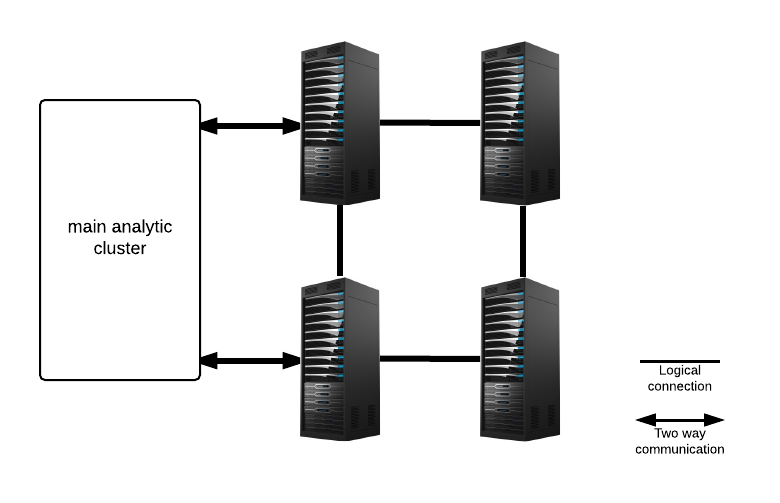
\includegraphics[width=0.7\textwidth]{6-hardware/images/db-cluster.png}
\caption{Logical schematic of storage cluster of HEMS}
\label{fig:database-cluster}
\end{figure}

As can be seen in \autoref{fig:database-cluster}, HEMS will use four database racks to have redundancy in the system. The server is connected as a ring, which is the common way to setup database server. By using this form of architecture, HEMS will be more reliable and fault tolerant. There will also be two physical connection to the main analytic cluster to make this system more fault tolerant in terms of connection. HEMS database cluster will use the same server, Dell PowerEdge R530, for controlling the SATA storage machine.

\subsection*{Related patterns}
This storage cluster implements broker, shared repository, and unit of work patterns. Broker pattern is implemented in a mechanism that any other component of this system can connect to the cluster and see this as a single entity, although actually the cluster consists of more than one entity. If this storage cluster is seen as a single entity, then this is also an implementation of shared repository pattern, where a client or other instance connects to the storage cluster and proceeds with corresponding operations. Unit of Work pattern will be used to keep track of changes to objects and to coordinate writing these changes to the database in one database call.

\subsection{Compute cluster}
\label{subsec:analytics}
Compute cluster will be the main brain of HEMS. The data presentation will be handled by this system. The analysis process also runs on top of this hardware. To increase availability and reliability, HEMS will have six server racks to do the processing as depicted in \autoref{fig:analytic-cluster}.

\begin{figure}[H]
\centering
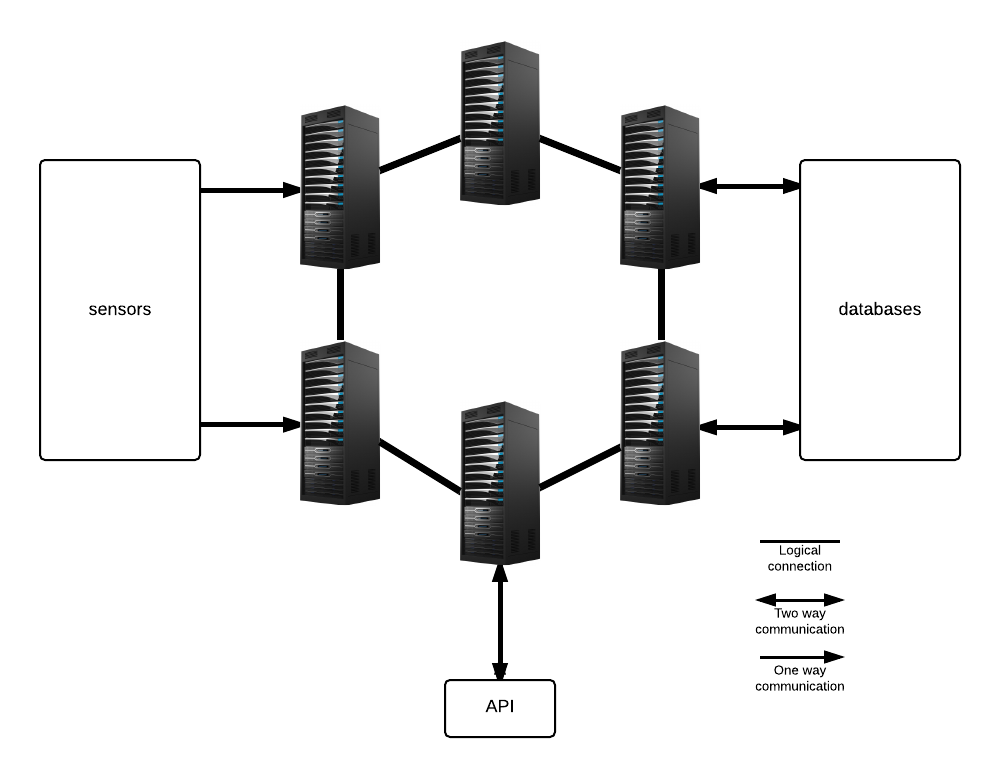
\includegraphics[width=0.7\textwidth]{6-hardware/images/analytic-cluster.png}
\caption{Logical schematic of analytic cluster of HEMS}
\label{fig:analytic-cluster}
\end{figure}

\subsection*{Related patterns}
Front page controller pattern is implemented in the compute cluster, which includes decorator and command pattern, because the compute cluster is also responsible for handling incoming connection through API. 

% !TEX root = ../report.tex
\chapter{Software Architecture}
\label{ch:software}

\section{Layer decomposition}

\begin{figure}[H]
\centering
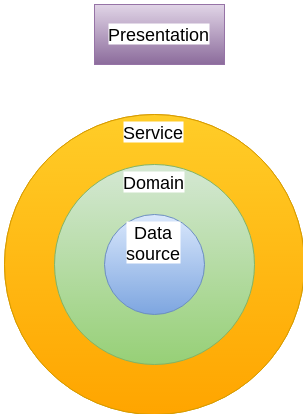
\includegraphics[scale=0.7]{7-software/images/LayersCircle.png}
\caption{Layer decomposition}
\label{fig:layerscircle}
\end{figure}

The system is decomposed into the following layers:
\begin{itemize}
\item Presentation Layer
\item Service Layer
\item Domain Layer
\item Data Source Layer
\end{itemize}

The presentation layer presents a view to the user. A user can use web browser and visit the energy monitoring website. The browser will then show a GUI to the user showing his energy statistics.\\

%TODO describe each layer
% The abc layer ...
% form vol4:
%%%% identify five different layers:
%%%•
%%% Presentation. This layer contains the interfaces to systems at the operation level of the automation pyramid, the so-called ‘north-bound gateways,’ as well as user-level applications that access the
%%%system’s functionality directly, such as for picking and warehouse
%%%topology management.
%%%•
%%% Business process. This layer provides the administrative and oper-
%%%ational functionality the system must support, such as stock
%%%management, order management, shipping, receiving, and material
%%%flow control.
%%%• Business objects. This layer comprises representations of domain-specific physical and logical entities on which the functionality in the business process layer operates. The main responsibility of this layer is to maintain and provide access to the warehouse topology.



Figure~\ref{fig:layersflow} shows these layers and includes their responsibilities and concerns. The communication between the boxes is how the concerns are connected to each other. It is not how the actual flow of communication is handled, the communication flow will be discussed in detail later.
%abc, add ref to communication layer thingy.

\begin{figure}[H]
\centering
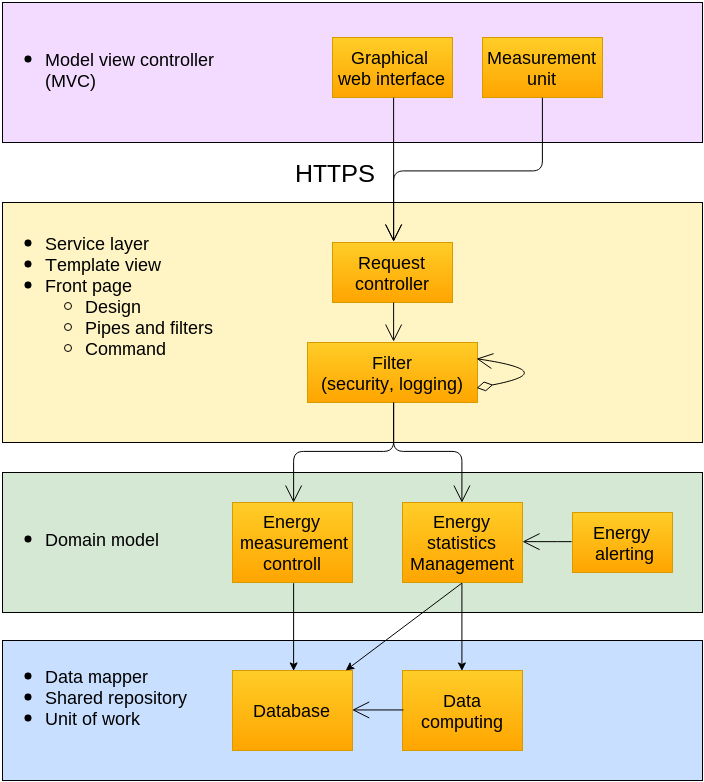
\includegraphics[scale=0.45]{7-software/images/layersflow.png}
\caption{Functionality of the system in each layer}
\label{fig:layersflow}
\end{figure}

Notice that the broker isn't mentioned. This is because the broker pattern is a pattern that handles the communication between the layers, which will be discussed in a later section.
%TODO add reference

\clearpage
\section{Data flow and transformation}

\begin{figure}[H]
\centering
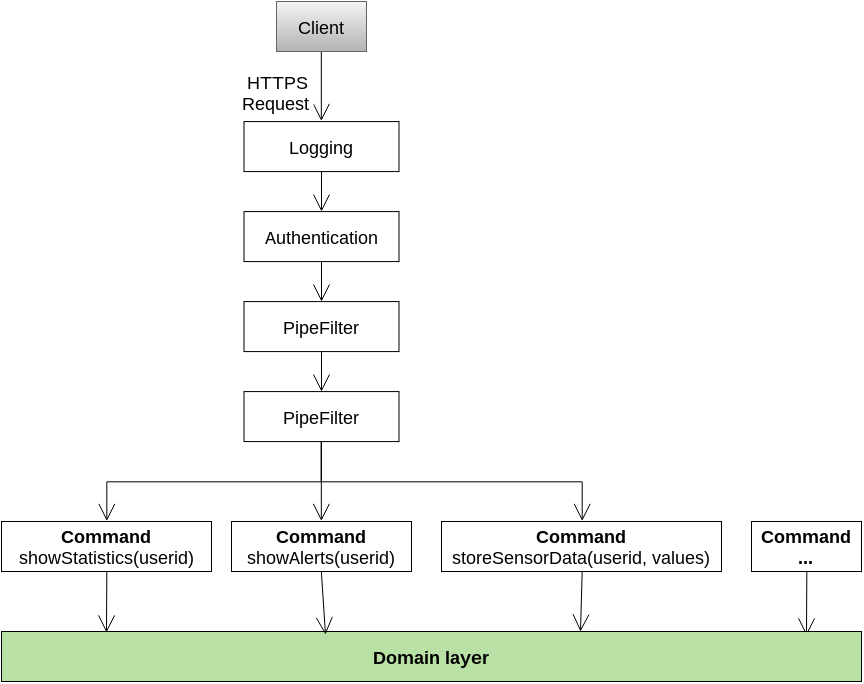
\includegraphics[width=0.8\linewidth]{7-software/images/FrontFlow.png}
\caption{Figure showing requests are piped and dispatched}
\label{fig:frontflow}
\end{figure}

\begin{figure}[H]
\centering
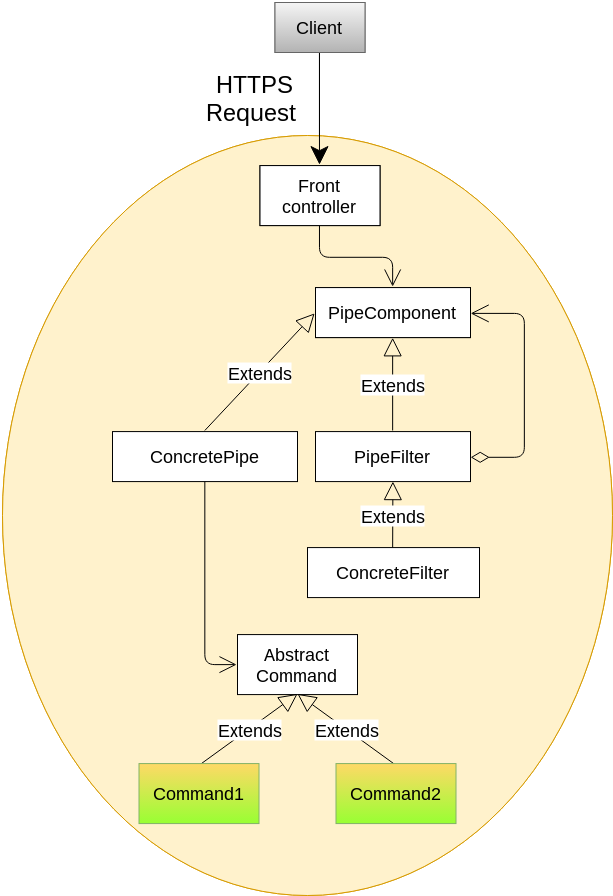
\includegraphics[width=0.5\linewidth]{7-software/images/FrontClasses.png}
\caption{Class diagram of the font page controller creating the pipes and filters}
\label{fig:frontclasses}
\end{figure}

\clearpage
\section{Data repository}

There are multiple components accessing a central repository of data. They do this by creating a query object and passing this to the repository. 
%TODO finish description

\begin{figure}[H]
\centering
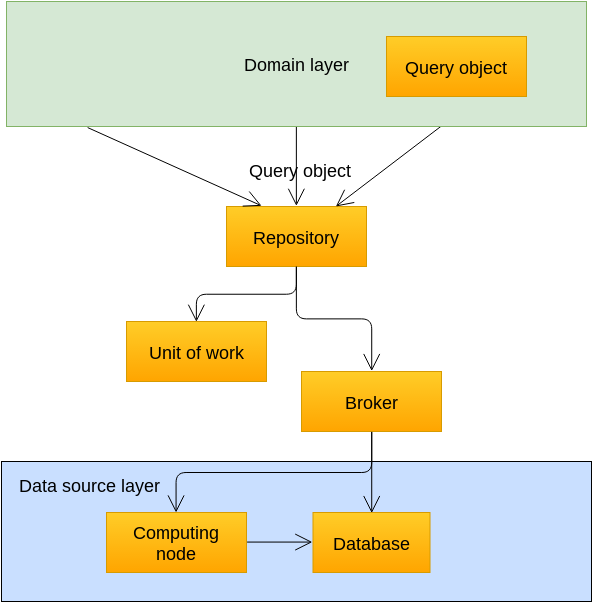
\includegraphics[width=0.6\linewidth]{7-software/images/RepoUowBroker.png}
\caption{Connection between domain layer and data source layer}
\label{fig:frontclasses}
\end{figure}

%TODO explain broker here

The Unit of Work pattern is used to keep track of the changes made to objects and newly created objects. Whenever an object is created, changed or deleted, the Unit of Work is told about this. 
Whenever the object can be saved to the database, the \verb|commit()| method of the Unit of Work is called, which translates the stored changes into database transactions.

A sequence diagram showing an example of this can be seen in Figure~\ref{fig:unitofworkseq}. 
This is an example of the user configuring the system. Here, the StatisticsController constructs a new Device object, which is fetched from the database and then registers itself with the Unit of Work. When the StatisticsController changes the name of this device, the device object registers itself as dirty with the Unit of Work. 
When the device object is saved, it calls \verb|commit()| on the Unit of Work, which leads to the device updating the appropriate fields in the database.

%TODO change the seq. diagram?? (add query object and call to broker?))
\begin{figure}[H]
\centering
\includegraphics[scale=0.7]{7-software/images/UnitOfWorkSeq.png}
\caption{Sequence diagram showing an update to a Device-object using Unit of Work}
\label{fig:unitofworkseq}
\end{figure}

\section{Interaction decoupling}

As mentioned in chapter \ref{ch:analysis}, MVC pattern is applied to decouple user-interface and the logic behind it. In this way, reusability is increased because the same models or controllers can be coupled with the same view. Modifiability is also increased because it becomes easier to modify a particular user interface or data model without interfering the logic, and vice-versa. Figure \ref{fig:mvc-architecture} depicts an example of MVC implementation in the HEMS.

\begin{figure}[H]
	\centering
	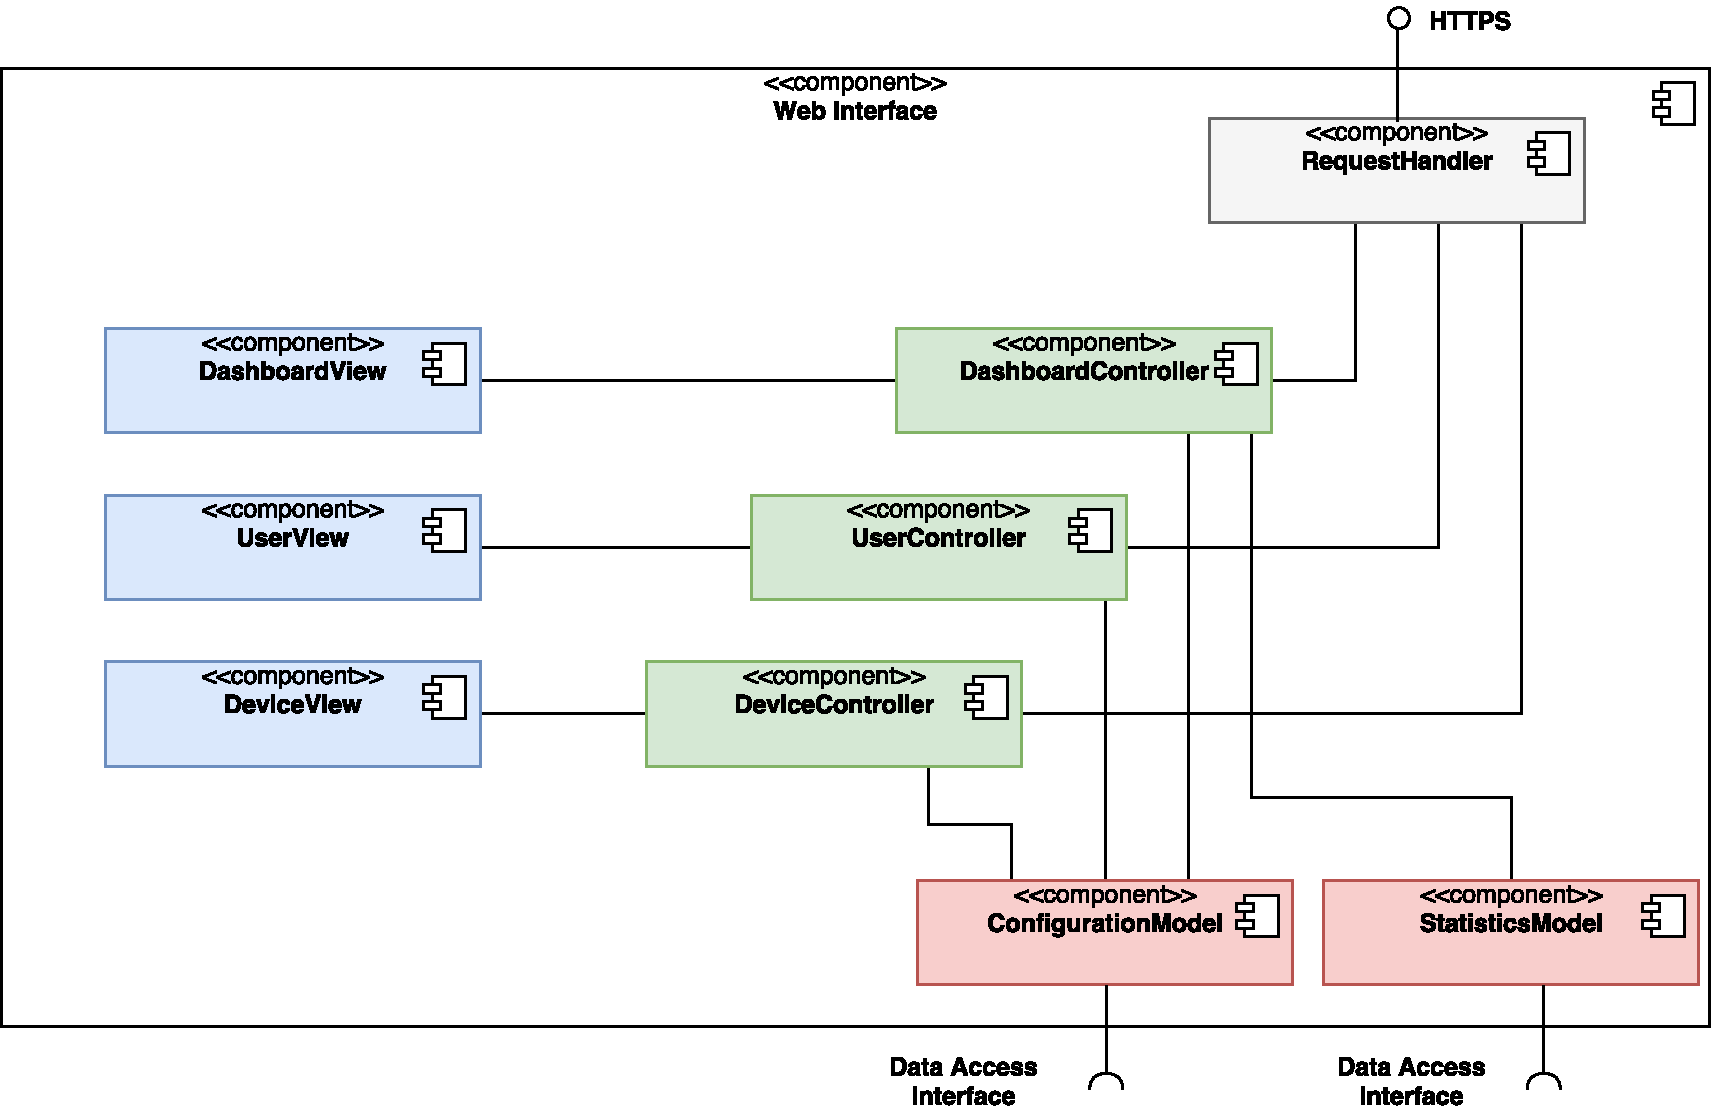
\includegraphics[width=0.8\textwidth]{7-software/images/mvc.pdf}
	\caption{Model-view-controller pattern implementation}
	\label{fig:mvc-architecture}
\end{figure}

\section{Component interaction}

\begin{figure}[H]
\centering
\includegraphics[scale=0.4]{7-software/images/Component.png}
\caption{The Layers}
\label{fig:layers}
\end{figure}

%TODO Possible describe client server?....

%TODO is this needed?:
%\section{Distributed communication}
%%- Broker
%%- RPC
%%- Message queue


\section{Summary}

%TODO add the challanges.
%like on posa v4 p93
\begin{table}[H]
	\pgfplotstabletypeset[%
		KeyValue
	]{%
	key & value\\
	\textbf{Pattern} & \textbf{Challenges} \\
	\midrule
	Layers & \\
	Model-View-Controller & \\
	Template view & \\
	Service Layer & \\
	Front page & \\
	Domain model & \\
	Unit of work & \\
	Broker & \\
	Data mapper & \\
	Repository & \\
	}
\caption{UC-\arabic{uc}: Configuration- adding new devices}
\label{table:patternchallenges}
\end{table}

%% !TEX root = ../report.tex

\section{Views}
The following section will elaborate the two of the `4$+$1 model' views of the system, namely the Logic View and the Process View.

\subsection{Logic view}

\subsection{Process view}
%
%% !TEX root = ../report.tex

\clearpage
\section{Elaborated model with patterns}
This section will describe the elaborated model on the basis of the patterns used in the architecture. For each patterns, this section will describe how it is implemented and how it affects the quality attributes of the system.

\subsection{Layers pattern}
\begin{figure}[H]
\centering
\includegraphics[scale=0.4]{7-software/images/Layers.png}
\caption{The Layers}
\label{fig:layers}
\end{figure}
The system is divided into four layers. The first layer is the presentation layer. This layer is responsible for handling the interaction with the end user. It contains the Web Interface, which is accessible to the user over HTTPS.

The second layer is the Service Layer, see Section~\ref{sec:service-layer-pattern} for more information about this layer. This layer offers services, which can be used by other (external) components.

The third layer is the Domain Layer and is responsible for the domain logic. The Domain Model contains all the classes, has an in-memory representation of the data and contains the logic which is inherent to the objects.
It uses the Unit of Work pattern (see Section~\ref{sec:unit-of-work-pattern}) to keep track of the changes to objects, so not every change will lead to a new database call. \\
The components in the Domain Layer are connected to the Domain Model, so they have access to the classes in there. \\
The Alerting component is responsible for sending alerts by email to the end user, for which it depends on an external Email Gateway. It also uses the StatisticsService in order to compute statistics, which it needs to decide if the user should be alerted by email. \\
The Configuration and Statistics components expose their functionality to the Service Layer.
% gateway is actually also a pattern :o

The Data Source layer contains the Unit of Work, which keeps track of the changes to the objects and translates those changes to database transactions when the object is committed. The layer also contains a Database Driver, which handles the communication with the database.

%TODO explain individual components (in one of the views?)


\subsection{Service Layer pattern}
\label{sec:service-layer-pattern}
The service layer encapsulates the application's business logic and defines the set of available operations/interfaces to clients. In Figure~\ref{fig:layers}, the Service Layer and its components can be seen. 

It contains the `StatisticsService', which exposes an interface used by clients to store the electricity usage data and is also used by the Web Interface for computing statistics. It is also used by the Alerts component in the Domain Layer, since it needs the same computed statistics as are displayed in the web interface, to decide if the user should be alerted by email.

The Service Layer also has the `Configuration Service', which is used by the Web Interface to allow the user to add new devices, change their properties or to configure new alerts.

The Service Layer makes a common set of application functionality available to many kinds of clients. This promotes the interoperability and also prevents having duplicate code.

\subsection{Front page}
In the figure below, the structure of the front page pattern is shown, which uses the decorator and command pattern.
\label{sec:unit-of-work-pattern}
\begin{figure}[H]
\centering
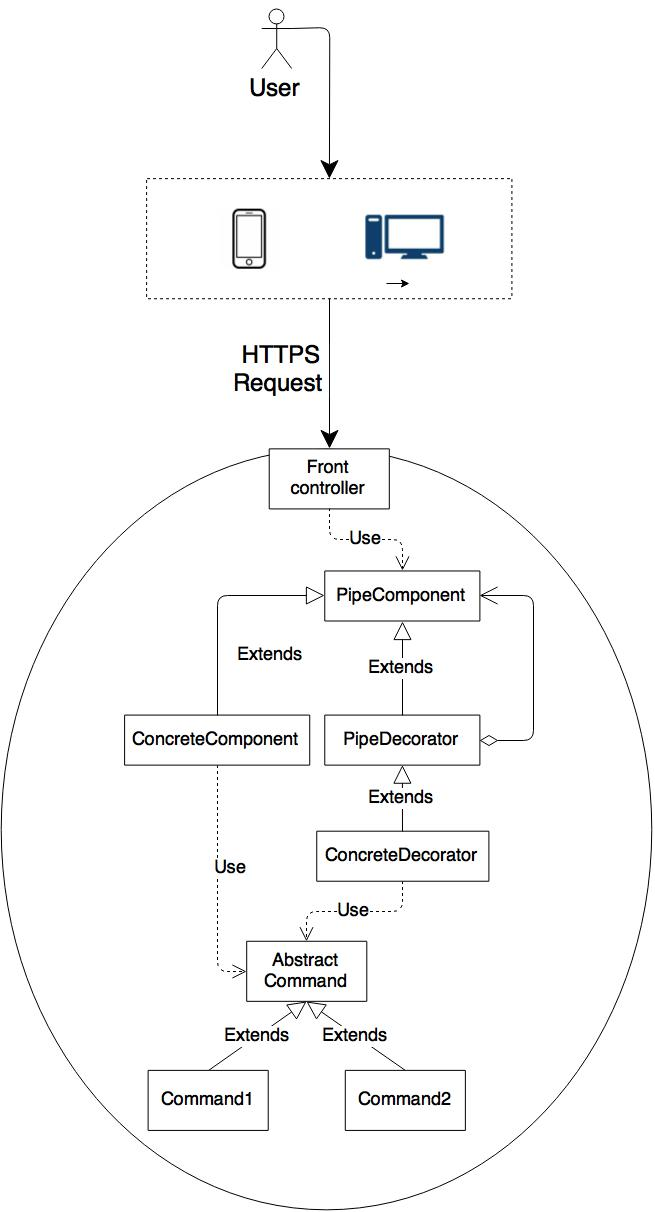
\includegraphics[scale=0.8, height=20cm]{7-software/images/frontPage.jpg}
\caption{The front controller}
\label{fig:frontcontroller}
\end{figure}

\clearpage
\subsection{Model-View-Controller}
\label{sec:mvc}
As mentioned in chapter \ref{ch:analysis}, MVC pattern is applied to decouple user-interface and the logic behind it. In this way, reusability is increased because the same models or controllers can be coupled with the same view. Modifiability is also increased because it becomes easier to modify a particular user interface or data model without interfering the logic, and vice-versa. Figure \ref{fig:mvc-architecture} depicts an example of MVC implementation in the HEMS.

\begin{figure}[H]
	\centering
	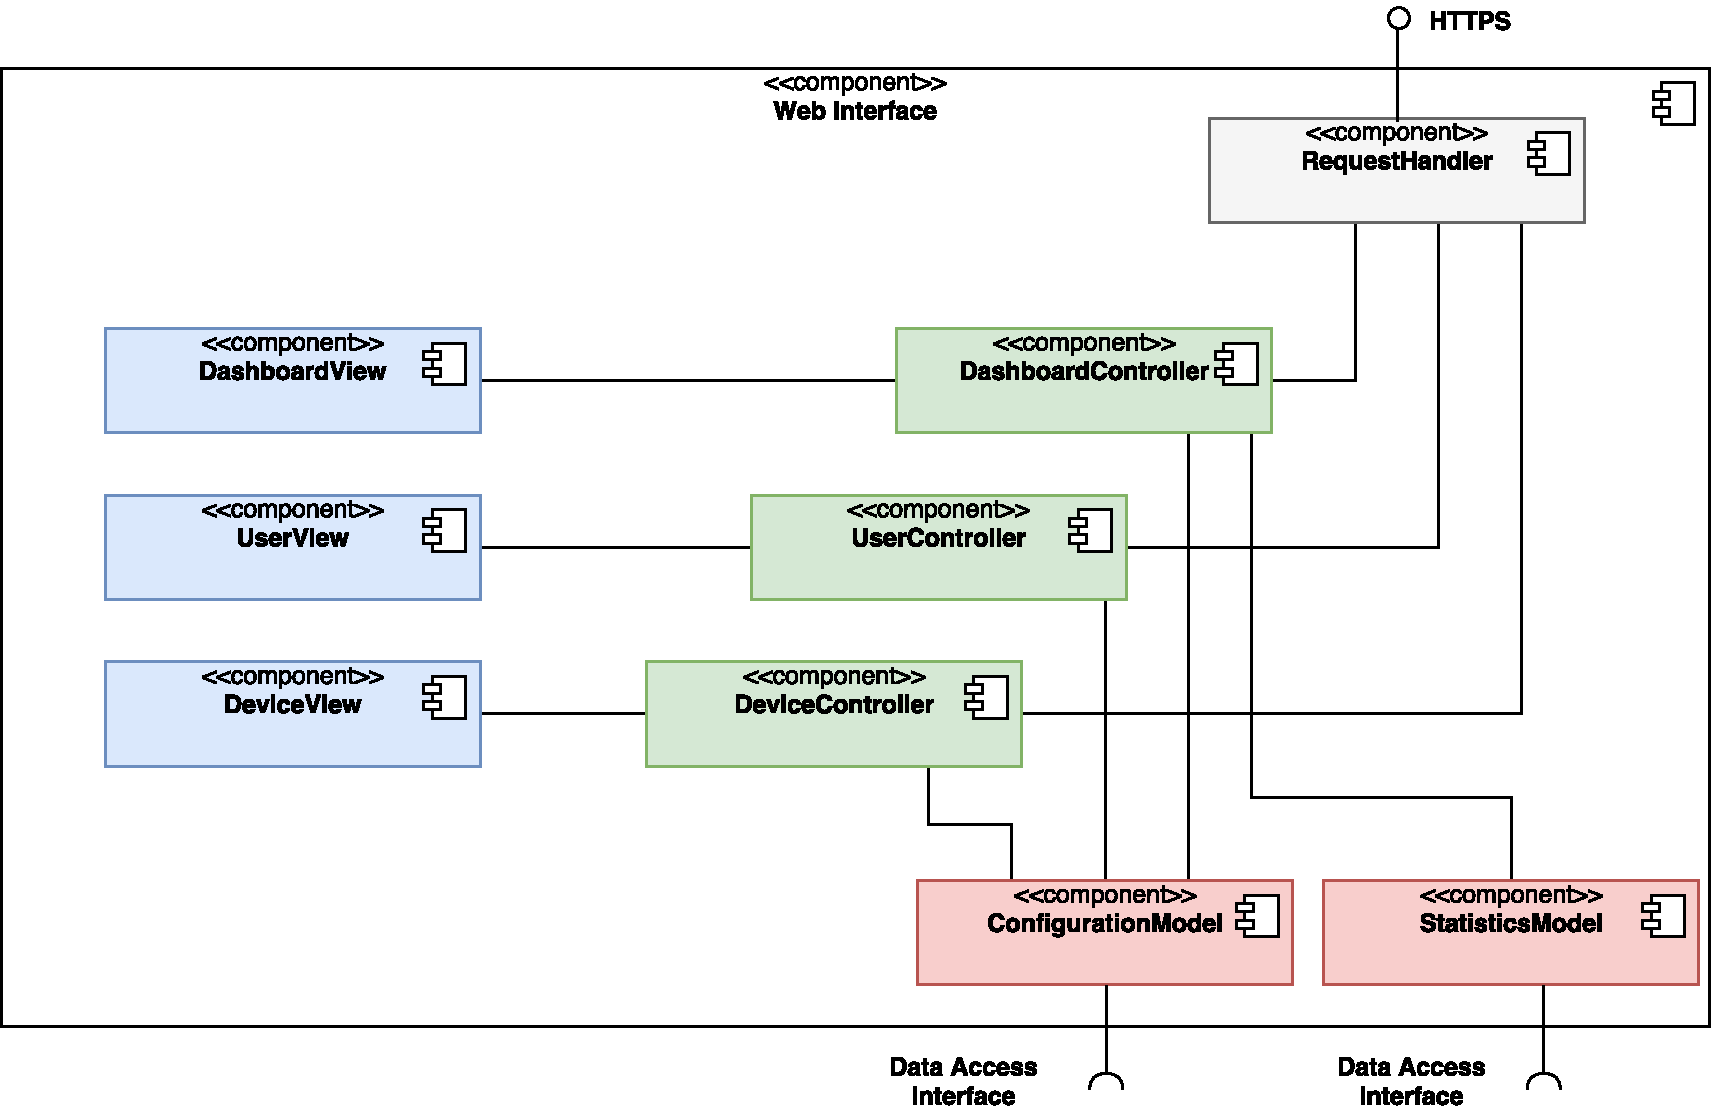
\includegraphics[width=0.8\textwidth]{7-software/images/mvc.pdf}
	\caption{Model-view-controller pattern implementation}
	\label{fig:mvc-architecture}
\end{figure}

Some models, views, and controllers are depicted in Figure \ref{fig:mvc-architecture}. Request handler handles incoming user request via HTTPS and routes it to the corresponding controller. Required data is then obtained through the models. Suitable views are used to provide user interface to the user. Some models, views, and controllers are presented in Figure \ref{fig:mvc-architecture}. However, there are more models, views, and controllers than those which are represented in the Figure \ref{fig:mvc-architecture}.

\clearpage
\subsection{Template View}
\label{sec:template-view}
Template view is implemented in this system to make the HTML code reusable in different pages. This will also make the view structure more simple. Code duplication can be prevented because instead of duplicating the code, the HTML will use a certain template.

\begin{figure}[H]
	\centering
	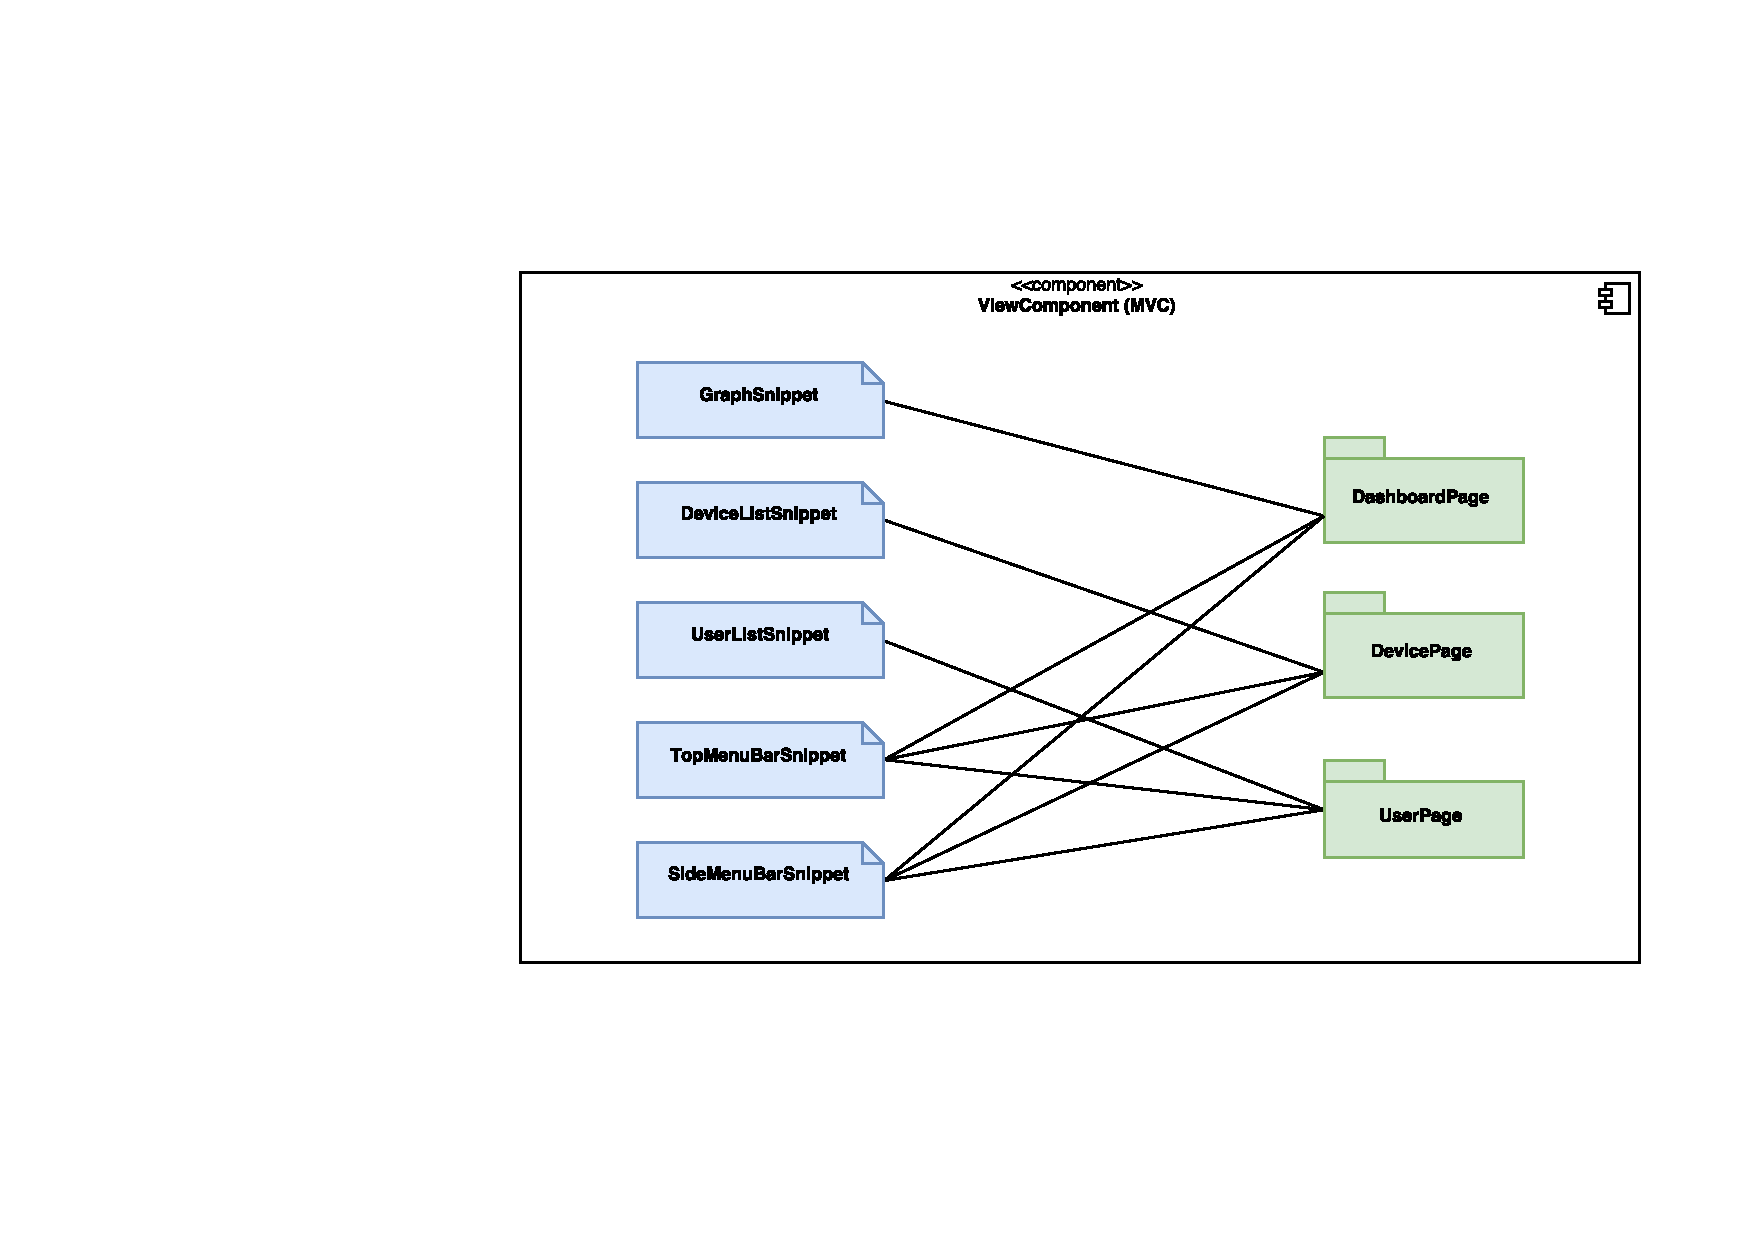
\includegraphics[width=0.7\textwidth]{7-software/images/template-view.pdf}
	\caption{Template view pattern implementation}
	\label{fig:template-view-architecture}
\end{figure}

Figure \ref{fig:template-view-architecture} shows an example of implementation of the template view pattern. Each page of the system (presented in green color) will combine several HTML code snippets (presented in blue color) together. \texttt{TopMenuBarSnippet} and \texttt{SideMenuBarSnippet} are used several times, as each page contains top menu bar and side menu bar. This is also good for expandability because the new page may just combine existing page template to create new web page.






%!TEX root = ../report.tex

\newcommand{\bo}[1]{\textbf{#1}}

\chapter{Architecture evaluation}
\label{ch:evaluation}

In this chapter the architecture of the system will be evaluated. After taking architectural decisions and building the system the architects have to make sure that the patterns applied suit the architecture, especially the quality attributes and key drivers .%in terms of benefits and liablities.


\paragraph{Layers}
\paragraph{Service Layer}
\paragraph{Front-Controller}
\paragraph{Domain Model}
\paragraph{Model View Controller}
\paragraph{Unit of Work}
\paragraph{Shared Repository} 
%Repositories are the single point where we hand off and fetch objects. It is also the boundary where communication with the storage starts and ends.
%Mediates between the domain and the data mapping layers using a collection-like interface for accessing domain objects.

\textit{Benefits} \\

The repository gives a lot more control over how the data is handled. The benefits are:
\begin{itemize}
\item Reduces code (and code complexity)
\item Increases performance
\item Separated domain and data layers, increasing flexibility and changeability
\end{itemize}

Performing analysis on the data also consists of executing complex queries on the data source. The database that executes these queries, however, might change. Or the system might decide to use multiple databases and data sources.
Using the Repository pattern, these changes can \underline{be made fast}. The repository also allows for \underline{multiple configurations} to exist. So an extra repository could be created for testing purposes, only using an in-memory database to increase the test execution speed. \\

\textit{} Liabilities : \\
\textbf{+ Reusability} \\
\textbf{+ Integrability} \\
\textbf{+ Modifiability/Changeability} by the Separation of concerns\\


\section{Requirements validation}
\label{sec:req-validation}
%!TEX root = ../report.tex
\subsection{Functional requirements}
\label{sec:fr-validation}
Functional requirements evaluation is depicted in Table \ref{table:eval-functional-requirements} below.

\begin{longtable}{lllL{\tw{0.2}}L{\tw{0.4}}}
    \bo{Nr.} & \bo{Priority} & \bo{Fulfilled} & \bo{Pattern(s)} & \bo{Remarks} \\ \toprule \endhead

 	% {receive-usage}{Must}
	% { The system must be able to receive electricity usage data from devices. }
    ~\ref{fr:receive-usage} 
    & Must     
    & Yes
    & ~\ref{sec:layers}
    & Receving data is handled by the layers pattern. The process starts with reception of sensor data from service layer, then the data is forwarded to domain layer to perform several failure checks. Lastly, the data is stored through data-source layer. \\ \midrule

 	% {store-usage}{Must}
	% { The system must be able to store electricity usage data. }
	~\ref{fr:store-usage} 
    & Must     
    & Yes
    & ~\ref{sec:unit-of-work}, \ref{sec:data-source-layer}, \ref{sec:repository}
    & Storing the data is mainly handled in data-source layer. This layer receives the data from the domain-layer. Unit of Work keeps track of changes to objects and coordinates storing the data to the database in one database call. The data is stored in single repository, so to say. \\ \midrule
	
	% {retrieve-usage}{Must}
	% { The system must be able to retrieve previously stored electricity usage data. }
	~\ref{fr:retrieve-usage} 
    & Must
    & Yes
    & ~\ref{sec:unit-of-work}, \ref{sec:data-source-layer}, \ref{sec:repository}
    & Previously stored data is available in the repository, which belongs to data-source layer. Unit of Work also keeps track of changes to objects. \\ \midrule
	
	% {compute-total}{Must}
	% { The system must be able to compute the total electricity consumption for a given time period for a particular house. }
	~\ref{fr:compute-total} 
    & Must     
    & Yes
    & ~\ref{sec:broker}, \ref{sec:layers}, \ref{sec:unit-of-work}
    & Computation process involves multiple pattern: domain and data-source layer. This process is also a high read-write process, thus unit of work pattern is useful for tracking the changes of objects and coordinates read/write process to the database. Broker makes sure that the parallel computation is taken care properly. \\ \midrule
	
	% {compute-timeperiod}{Must}
	% { The system must be able to compute the electricity consumption per device for a given time period. }
	~\ref{fr:compute-timeperiod} 
    & Must     
    & Yes
    & ~\ref{sec:broker}, \ref{sec:layers}, \ref{sec:unit-of-work}
    & This process is also similar with previous process (\ref{fr:compute-timeperiod}), but this is more time-range restricted. \\ \midrule
	
	% {compute-bill}{Must}
	% { The system must be able to compute an estimated electricity bill for the current month based on the electricity consumption to that point. }
	~\ref{fr:compute-bill} 
    & Must     
    & Yes
    & ~\ref{sec:broker}, \ref{sec:layers}, \ref{sec:unit-of-work}
    & Computing bill process involves multiple pattern: domain and data-source layer. This process is also a high read-write process, thus unit of work pattern is useful for tracking the changes of objects and coordinates read/write process to the database. Broker makes sure that the parallel computation is taken care properly. \\ \midrule
	
	% {interface-selectstats}{Must}
	% { A user of the system must be able to select which statistics to compute in a web interface. }
	~\ref{fr:interface-selectstats} 
    & Must     
    & Yes
    & ~\ref{sec:mvc-analysis}, \ref{sec:template-view-analysis}
    & All operations done in web interface are taken care by the template view and MVC pattern. \\ \midrule
	
	% {web-interface}{Must}
	% { The system must be able to show the computed statistics in a web interface. }
	~\ref{fr:web-interface} 
    & Must     
    & Yes
    & ~\ref{sec:mvc-analysis}, \ref{sec:template-view-analysis}
    & All operations done in web interface are taken care by the template view and MVC pattern.\\ \midrule
	
	% {interface-register}{Must}
	% { The system must allow users to register an account on the web interface. }
	~\ref{fr:interface-register} 
    & Must     
    & Yes
    & ~\ref{sec:front-page}, \ref{sec:mvc-analysis}, \ref{sec:template-view-analysis}
    & Registration, which is done through web interface, is taken care by the template view and MVC pattern as well. The front page will handle the logging, authentication and initial security of the request. \\ \midrule
	
	% {interface-login}{Must}
	% { The system must require users to be logged in, before the user can view electricity usage information about his/her house. }
	~\ref{fr:interface-login} 
    & Must     
    & Yes
    & ~\ref{sec:front-page}, \ref{sec:mvc-analysis}, \ref{sec:template-view-analysis}
    & The front page will handle the logging, authentication and initial security of the request. User interface is provided through MVC and template view pattern. \\ \midrule
	
	% {add-house}{Must}
	% { A user of the system must be able to register a new house using the web interface. }
	~\ref{fr:add-house} 
    & Must     
    & Yes
    & ~\ref{sec:front-page}, \ref{sec:mvc-analysis}, \ref{sec:template-view-analysis}
    & In order to add a house, a user must be logged in. The front page will handle the logging, authentication and initial security of the request. User interface is provided through MVC and template view pattern. \\ \midrule
	
	% {add-device}{Must}
	% { A user of the system must be able to register a new device for his house using the web interface. }
	~\ref{fr:add-device} 
    & Must
    & Yes
    & ~\ref{sec:front-page}, \ref{sec:mvc-analysis}, \ref{sec:template-view-analysis}
    & In order to add a device, a user must be logged in. The front page will handle the logging, authentication and initial security of the request. User interface is provided through MVC and template view pattern. \\ \midrule
	
	% {configure-price}{Must}
	% { A user of the system must be able to configure the price of a kWH in the web interface. }
	~\ref{fr:configure-price} 
    & Must     
    & Yes
    & ~\ref{sec:front-page}, \ref{sec:mvc-analysis}, \ref{sec:template-view-analysis}
    & In order to configure the price of the electricity, a user must be logged in. The front page will handle the logging, authentication and initial security of the request. User interface is provided through MVC and template view pattern. \\ \midrule
	
	% {feedback}{Must}
	% { The system must be able to send feedback to registered devices about the current electricity usage. }
	~\ref{fr:feedback} 
    & Must     
    & Yes
    & ~\ref{sec:layers}, \ref{sec:service-layer}
    & This is multi-tier operation, which involves all layers. The feedback is sent through the service layer. \\ \midrule
	
	% {show-accuracy}{Must}
	% { The system must be able to take the inaccuracy of the sensors into account when computing the statistics. }
	~\ref{fr:show-accuracy} 
    & Must     
    & Yes
    & ~\ref{sec:layers}, \ref{sec:domain-layer}, \ref{sec:unit-of-work}
    & The accuracy is provided by the sensor itself. The computation process is taken care in the domain layer. \\ \midrule
	
	% {show-history}{Must}
	% { The system must be able to display the history of electricity usage. }
	~\ref{fr:show-history} 
    & Must     
    & Yes
    & ~\ref{sec:mvc-analysis}, \ref{sec:template-view-analysis}
    & The history, computed in \ref{fr:retrieve-usage}, is shown to the user through web interface, which involves MVC and template view pattern. \\ \midrule
	
	% {choose-alerts}{Should}
	% { Users of the system should be able to subscribe to alerts in the web interface, alerting them about sudden energy increases or when they are using more energy than in previous months/weeks. }
	~\ref{fr:choose-alerts} 
    & Should     
    & Yes
    & ~\ref{sec:mvc-analysis}, \ref{sec:template-view-analysis}
    & The alert is shown in the web interface, which employs MVC and template view pattern. \\ \midrule
	
	% {alerts}{Should}
	% { The system should send alerts to users by mail when the user is subscribed for this alert and the condition for the alert is met. }
	~\ref{fr:alerts}
    & Should     
    & Yes
    & ~\ref{sec:layers}, \ref{sec:domain-layer}
    & This is a multi-tier operation, which includes domain and service layer. The email is sent through service layer. \\ \midrule
	
	% {interface-graph}{Should}
	% { The system should be able to show the computed statistics in a graph. }
	~\ref{fr:interface-graph} 
    & Should
    & Yes
    & ~\ref{sec:mvc-analysis}, \ref{sec:template-view-analysis}
    & Graph is shown in the web interface, which employs MVC and template view pattern. \\\bottomrule		

    \caption{Evaluation of functional-requirements}
    \label{table:eval-functional-requirements}
\end{longtable}
%!TEX root = ../report.tex
\subsection{Non-Functional requirement}
\label{sec:nfr-validation}
This subsection presents non-functional requirements evaluation in tables.

\subsubsection{Usability}

\begin{longtable}{llL{\tw{0.2}}L{\tw{0.4}}}
    \bo{Nr.} & \bo{Fulfilled} & \bo{Pattern(s)} & \bo{Remarks} \\ \toprule \endhead
	
	% \reqRow{US}{app}{An application is available for tablets and phone with those OS Windows Phone, Android, and iPhone.} \\
	~\ref{US:app}
    & Yes
    & ~\ref{sec:mvc-analysis}, \ref{sec:template-view-analysis}
    & Fulfilled with web application, which employs MVC and template view pattern. \\
	\midrule
	% \reqRow{US}{basic-understanding}{The end-user needs maximum ten minutes to get a basic understanding of system features through the UI. }\\
	~\ref{US:basic-understanding}
    & Yes
    & ~\ref{sec:mvc-analysis}, \ref{sec:template-view-analysis}
    & Fulfilled by using MVC and template view pattern. \\
	\midrule
	% \reqRow{US}{spa}{Every feature/major option of the system can be accessed through the home page (Single Page Application). }\\
	~\ref{US:spa}
    & Yes
    & ~\ref{sec:mvc-analysis}, \ref{sec:template-view-analysis}
    & Fulfilled by using MVC and template view pattern. \\
    \bottomrule		

    \caption{Evaluation of non-functional requirements: usability}
    \label{table:eval-usability}
\end{longtable}

\subsubsection{Reliability}

\begin{longtable}{llL{\tw{0.2}}L{\tw{0.4}}}
    \bo{Nr.} & \bo{Fulfilled} & \bo{Pattern(s)} & \bo{Remarks} \\ \toprule \endhead
	
	% \reqRow{RE}{error-margin}{A margin of error of $5\%$ in the energy measurements is tolerated.} \\
	~\ref{RE:error-margin}
    & No
    & -
    & Sensor accuracy is out of scope of this project as this project does not deal with sensor hardware. \\
	\midrule
	% \reqRow{RE}{availability}{The system should be available $99.9\%$. of the time which means down for 44 minutes within 6 months.}\\
	~\ref{RE:availability}
    & Yes
    & ~\ref{sec:layers}, \ref{sec:service-layer}, \ref{sec:unitofwork}, \ref{sec:broker}
    & High availability is achieved by separating the service in layers and parallelizing the processes.\\
	\midrule
	% \reqRow{RE}{downtime}{The system should be down for maximum ten minutes when the user installs a new release (version).}\\
	~\ref{RE:downtime}
    & Yes
    & ~\ref{sec:layers}, \ref{sec:service-layer}, \ref{sec:unitofwork}, \ref{sec:broker}
    & Separated layers tame care smooth new version deployment in the HEMS.\\
    \bottomrule		

    \caption{Evaluation of non-functional requirements: reliability}
    \label{table:eval-reliability}
\end{longtable}

\subsubsection{Security}

\begin{longtable}{llL{\tw{0.2}}L{\tw{0.4}}}
    \bo{Nr.} & \bo{Fulfilled} & \bo{Pattern(s)} & \bo{Remarks} \\ \toprule \endhead
	
	% \reqRow{SEC}{login}{Each user is identified and has to log in in order to access his "Home Energy Monitor" account.} \\
	~\ref{SEC:login}
    & Yes
    & ~\ref{sec:front-page}, \ref{sec:mvc-analysis}, \ref{sec:template-view-analysis}
    & Login page is handled by MVC and template view pattern. Front page pattern also helps to serve the login request. \\
	\midrule
	% \reqRow{SEC}{encryption}{The data stored in the database is encrypted.}\\
	~\ref{SEC:encryption}
    & Yes
    & ~\ref{sec:repository}
    & Repository pattern is used to encrypt the data in the database.\\
	\midrule
	% \reqRow{SEC}{https}{The connection from/to the system is encrypted using secure connection.}\\
	~\ref{SEC:https}
    & Yes
    & ~\ref{sec:layers}, \ref{sec:service-layer}
    & Layers and service layer pattern make sure the connections are secured using HTTPS channel. \\
    \bottomrule		

    \caption{Evaluation of non-functional requirements: security}
    \label{table:eval-security}
\end{longtable}

\subsubsection{Interoperability}

\begin{longtable}{llL{\tw{0.2}}L{\tw{0.4}}}
    \bo{Nr.} & \bo{Fulfilled} & \bo{Pattern(s)} & \bo{Remarks} \\ \toprule \endhead
	
	% \reqRow{INT}{interface}{The web interface of the system is available and functioning for 95\% of the browser market share.} \\
	~\ref{INT:interface}
    & Yes
    & ~\ref{sec:mvc-analysis}, \ref{sec:template-view-analysis}
    & The web interface are mainly handled by MVC and template view pattern.\\
	\midrule
	% \reqRow{INT}{rest}{The system exposes a REST interface that allows different electricity usage sensors to submit the electricity usage data.}\\
	~\ref{INT:rest}
    & Yes
    & ~\ref{sec:layers}, \ref{sec:service-layer}
    & REST interface are exposed in service layer. \\
    \bottomrule		

    \caption{Evaluation of non-functional requirements: interoperability}
    \label{table:eval-interoperability}
\end{longtable}

\subsubsection{Scalability}

\begin{longtable}{llL{\tw{0.2}}L{\tw{0.4}}}
    \bo{Nr.} & \bo{Fulfilled} & \bo{Pattern(s)} & \bo{Remarks} \\ \toprule \endhead
	
	% \reqRow{SCA}{user}{The system should still perform as efficiently as it is suppose to be when the number of users doubled.} \\
	~\ref{SCA:user}
    & Yes
    & ~\ref{sec:layers}, \ref{sec:broker}, \ref{sec:unitofwork}, \ref{sec:datamapper}
    & The system uses layers which are possible to be replicated.\\
	\midrule
	% \reqRow{SCA}{device}{The system should still perform as efficiently as it is suppose to be when the number of devices doubled.}\\
	~\ref{SCA:device}
    & Yes
    & ~\ref{sec:layers}, \ref{sec:broker}, \ref{sec:unitofwork}, \ref{sec:datamapper}
    & The system uses layers which are possible to be replicated.\\
    \bottomrule		

    \caption{Evaluation of non-functional requirements: scalability}
    \label{table:eval-scalability}
\end{longtable}



%!TEX root = ../report.tex
\chapter{System evolution}
\label{ch:evolution}
Due to new environmental issues(global warming, etc) The Home Energy Monitoring is a market in expansion and building green-friendly systems has become an important issue nowadays. This is an opportunity for the HEMS to grow by adding new features in the years to come. \\
" Various studies have shown a reduction in home energy use of 4-15\%\ through use of home energy display " (Source : \textit{Wikipedia} ). This percentage show the efficiency and the impact on the everyday life of such systems and that more and more users will use them. 

 \paragraph{Monitoring other energy consumption}
 The system will access new API and data stores providing other external energy data like gas consumption for example. 

 \paragraph{Computing new analysis}
The system will allow the user to compute and display to the user his greenhouse gas emission for example.

 %\paragraph{Application}
 %in order to make the access to his interface easier for the user an application for Android, Windows Phone and iOS will be built.
  
 \paragraph{Home automation functionnalities}
Knowing how the user consumes is good but controlling it is even better. \\ One of the goal of HEMS is to make the user more energy efficient.
The website/application will allow the user to control devices remotely (turning them on/off or changing light luminosity or heating intensity for example). \\
Th system will be able to advice the user about his energy consumption (ex: you should turn off this light because the room is empty, etc).

%!TEX root = ../report.tex
%\cleardoublepage
%\clearpage
%
%\appendix
%\appendixpage
%\addappheadtotoc

\begin{appendices}
			
	%\addcontentsline{toc}{part}{\appendixname}
				
	\renewcommand{\thechapter}{\Alph{chapter}}
	\renewcommand{\thesection}{\thechapter.\arabic{section}}
	\renewcommand{\thesubsection}{\thesection.\arabic{subsection}}
	\renewcommand{\thesubsubsection}{\thesubsection.\arabic{subsubsection}}

	% !TEX root = ../report.tex
\chapter{Time Tracking}
\label{App: Time Tracking}

\section*{Week 1}

% STRUCTURE:
%\begin{longtable}{p{0.2\textwidth} p{0.7\textwidth} p{0.1\textwidth}}
%	\textbf{Person} & \textbf{Task} & \textbf{Hours} \\ \toprule
%	Putra           &	&	\\ \midrule
%	Fakambi         &	&	\\ \midrule
%	Schaefers       & 	& 	\\ \midrule
%	Menninga        &	&	\\ \bottomrule
%\end{longtable}

\begin{longtable}{p{0.2\textwidth} p{0.7\textwidth} p{0.1\textwidth}}
	\textbf{Person} & \textbf{Task} & \textbf{Hours} \\ \toprule
	Putra           & Meetings, writing introduction and system context.	& 4	\\ \midrule
	Fakambi         & Meeting, First approach on non functional requirements and risks & 4 \\ \midrule
	Schaefers       & Meetings, Added a stake holders and key drivers description.	& 	5 \\ \midrule
	Menninga        & Meeting, high-level and functional requirements and improvements to risks	&	5\\ \bottomrule
\end{longtable}

\section*{Week 2}

\begin{longtable}{p{0.2\textwidth} p{0.7\textwidth} p{0.1\textwidth}}
	\textbf{Person} & \textbf{Task} & \textbf{Hours} \\ \toprule
	Putra           & Meetings, editing introduction and adding hardware architecture.	& 5	\\ \midrule
	Fakambi         & Meetings , work on the use-cases & 6 \\ \midrule
	Schaefers       & Meetings, researched patterns to use and created initial analysis draft & 9\\ \midrule
	Menninga        & Meetings, system architecture, use case improvements & 8 \\ \bottomrule
\end{longtable}

\section*{Week 3}

\begin{longtable}{p{0.2\textwidth} p{0.7\textwidth} p{0.1\textwidth}}
	\textbf{Person} & \textbf{Task} & \textbf{Hours} \\ \toprule
<<<<<<< HEAD

	Putra           & Meetings, processing feedback, working on MVC and templave view patterns in analysis and software architecture chapter & \\ \midrule
	Fakambi         & Meetings,updated use-cases, work on the Shared repository pattern & \\ \midrule
	Putra           & Meetings, processing feedback, working on MVC and template view patterns in analysis and software architecture chapter & \\ \midrule
	Fakambi         & & \\ \midrule
>>>>>>> a20c0f2661ce7ed8ffee8fe4608230a569de449a
	Schaefers       & & \\ \midrule
	Menninga        & Meetings, feedback, working on Layers/Unit of Work/Service Layer patterns (ch. 3 \& 6) & 12.0 \\ \bottomrule
=======
	Putra           & Meetings, processing feedback, working on MVC and template view patterns in analysis and software architecture chapter & 12 \\ \midrule
	Fakambi         & Meetings,updated use-cases, work on the Shared repository pattern &  8 \\ \midrule
	Schaefers       & Meetings, researching patterns in the various books, describing front controller and command patterns& 14.0 \\ \midrule
	Menninga        & Meetings, feedback, working on Layers/Unit of Work/Service Layer patterns (ch. 3 \& 6), improved elaborated model & 13.0 \\ \bottomrule
>>>>>>> b1701830ab05a93008f873a1c15ff9a1536422aa
\end{longtable}

% \section*{Week 4}

% \begin{longtable}{p{0.2\textwidth} p{0.7\textwidth} p{0.1\textwidth}}
% 	\textbf{Person} & \textbf{Task} & \textbf{Hours} \\ \toprule
% 	Putra           & & \\ \midrule
% 	Fakambi         & & \\ \midrule
% 	Schaefers       & & \\ \midrule
% 	Menninga        & & \\ \bottomrule
% \end{longtable}
	
\end{appendices}

\bibliography{library}

\end{document}
